\documentclass[a4paper]{article}

% ##- In R -
% ## Sweave("bio3d_vignette.Rnw")
% ## tools::texi2dvi("bio3d_vignette.tex", pdf=TRUE)
% ##

\usepackage{natbib}
\usepackage{color}
\definecolor{myurlblue}{rgb}{0.3,0.2,0.7}
\usepackage[colorlinks=true,urlcolor=myurlblue,pagecolor=black,citecolor=myurlblue,linkcolor=black]{hyperref}


\title{An Introduction to the bio3d Package (Vignette 1)}
\author{Barry Grant\\
University of California, San Diego}



\usepackage{/net/home/bgrant/software/R-local/R-2.7.2/share/texmf/Sweave}
\begin{document}


\maketitle
\tableofcontents


\section{Introduction}
The aim of this document, termed a vignette\footnote{This vignette contains executable examples, see \texttt{help(vignette)} for further details.} in R parlance, is to provide a task-oriented introduction to the bio3d R package \citep{grant06}.  Bio3d contains utilities to process, organize and explore protein structure, sequence and dynamics data.  Features include the ability to read and write structure, sequence and dynamic trajectory data, perform atom selection, re-orientation, superposition, rigid core identification, clustering, torsion analysis, distance matrix analysis, structure and sequence conservation analysis, and principal component analysis.

In addition, various utility functions are provided to enable the statistical and graphical power of the R environment to work with biological sequence and structural data.  




\paragraph{Supporting Material:}
The latest version and further documentation can be obtained from the bio3d website: \href{http://mccammon.ucsd.edu/~bgrant/bio3d/}{http://mccammon.ucsd.edu/$\sim$bgrant/bio3d/} and wiki: \href{http://bio3d.pbwiki.com/}{http://bio3d.pbwiki.com/}.




\subsection{Getting Started}
Start R, load the bio3d package and use the command \texttt{lbio3d()} to list the current functions available within the package:

\begin{Schunk}
\begin{Sinput}
> library(bio3d)
> lbio3d()
\end{Sinput}
\begin{Soutput}
 [1] "aa123"             "aa2index"          "aa321"            
 [4] "aln2html"          "angle.xyz"         "atom2xyz"         
 [7] "atom.select"       "blast.pdb"         "bounds"           
[10] "bwr.colors"        "chain.pdb"         "cmap"             
[13] "consensus"         "conserv"           "convert.pdb"      
[16] "core.find"         "dccm"              "diag.ind"         
[19] "dist.xyz"          "dm"                "dm.xyz"           
[22] "dssp"              "entropy"           "fit.xyz"          
[25] "gap.inspect"       "get.pdb"           "get.seq"          
[28] "ide.filter"        "identity"          "is.gap"           
[31] "lbio3d"            "mktrj.pca"         "mono.colors"      
[34] "orient.pdb"        "pairwise"          "pca.project"      
[37] "pca.tor"           "pca.xyz"           "pca.xyz2z"        
[40] "pca.z2xyz"         "pdb.summary"       "plot.bio3d"       
[43] "plot.blast"        "plot.core"         "plot.dmat"        
[46] "plot.pca"          "plot.pca.loadings" "plot.pca.score"   
[49] "plot.pca.scree"    "print.core"        "read.all"         
[52] "read.crd"          "read.dcd"          "read.fasta"       
[55] "read.fasta.pdb"    "read.ncdf"         "read.pdb"         
[58] "read.pqr"          "rmsd"              "rmsd.filter"      
[61] "rmsf"              "rot.lsq"           "seqaln"           
[64] "seqaln.pair"       "seqbind"           "seq.pdb"          
[67] "split.pdb"         "store.atom"        "stride"           
[70] "torsion.pdb"       "torsion.xyz"       "trim.pdb"         
[73] "unbound"           "wiki.tbl"          "wrap.tor"         
[76] "write.crd"         "write.fasta"       "write.ncdf"       
[79] "write.pdb"         "write.pqr"        
\end{Soutput}
\end{Schunk}
Detailed documentation and example code for each function can be accessed via the \texttt{help()} and \texttt{example()} commands (e.g. \texttt{help(read.pdb)}).  You can also copy and paste any of the example code from the documentation of a particular function directly into your R session:

\begin{Schunk}
\begin{Sinput}
> pdb <- read.pdb(get.pdb("1bg2", URLonly = TRUE))
\end{Sinput}
\begin{Soutput}
  HEADER    MOTOR PROTEIN                           04-JUN-98   1BG2               
\end{Soutput}
\end{Schunk}
In the above example the \texttt{get.pdb()} command returns the RCSB Protein Data Bank file for structure \texttt{1bg2}.  Setting \texttt{URLonly} to \texttt{FALSE} would cause the file to be downloaded to the current working directory.  The \texttt{read.pdb()} command then processes this file and returns its output to the object \texttt{pdb}.  To examine the contents of the \texttt{pdb} object we can use the \texttt{attributes} command.

\begin{Schunk}
\begin{Sinput}
> attributes(pdb)
\end{Sinput}
\begin{Soutput}
$names
[1] "atom"   "het"    "helix"  "sheet"  "seqres" "xyz"    "calpha"

$class
[1] "pdb"
\end{Soutput}
\end{Schunk}
Most bio3d functions, including \texttt{read.pdb()}, return list objects whose components can be accessed in the standard way (see \texttt{help(read.pdb)} for further details).  For example, to print coordinate data for the first three atoms in our newly created \texttt{pdb} object type:

\begin{Schunk}
\begin{Sinput}
> pdb$atom[1:3, c("resno", "resid", "elety", "x", "y", "z")]
\end{Sinput}
\begin{Soutput}
     resno resid elety x        y        z       
[1,] "3"   "ASP" "N"   "43.743" "-2.106" "39.408"
[2,] "3"   "ASP" "CA"  "45.053" "-2.661" "39.856"
[3,] "3"   "ASP" "C"   "45.305" "-2.401" "41.340"
\end{Soutput}
\end{Schunk}
In the previous example we use numeric indices to access atoms 1 to 3. In a similar fashion the \texttt{atom.select()} function returns numeric indices that can be used for convinent data access: 
\begin{Schunk}
\begin{Sinput}
> inds <- atom.select(pdb, "calpha")
\end{Sinput}
\begin{Soutput}
      segid  chain  resno  resid  eleno  elety
Stest ""     ""     ""     ""     ""     "CA" 
Natom "2527" "2527" "2527" "2527" "2527" "323"
 *  Selected a total of: 323 intersecting atoms  *
\end{Soutput}
\begin{Sinput}
> plot.bio3d(pdb$atom[inds$atom, "resno"], pdb$atom[inds$atom, 
+     "b"], sse = pdb, ylab = "Bfactor", xlab = "Residue Number")
\end{Sinput}
\end{Schunk}
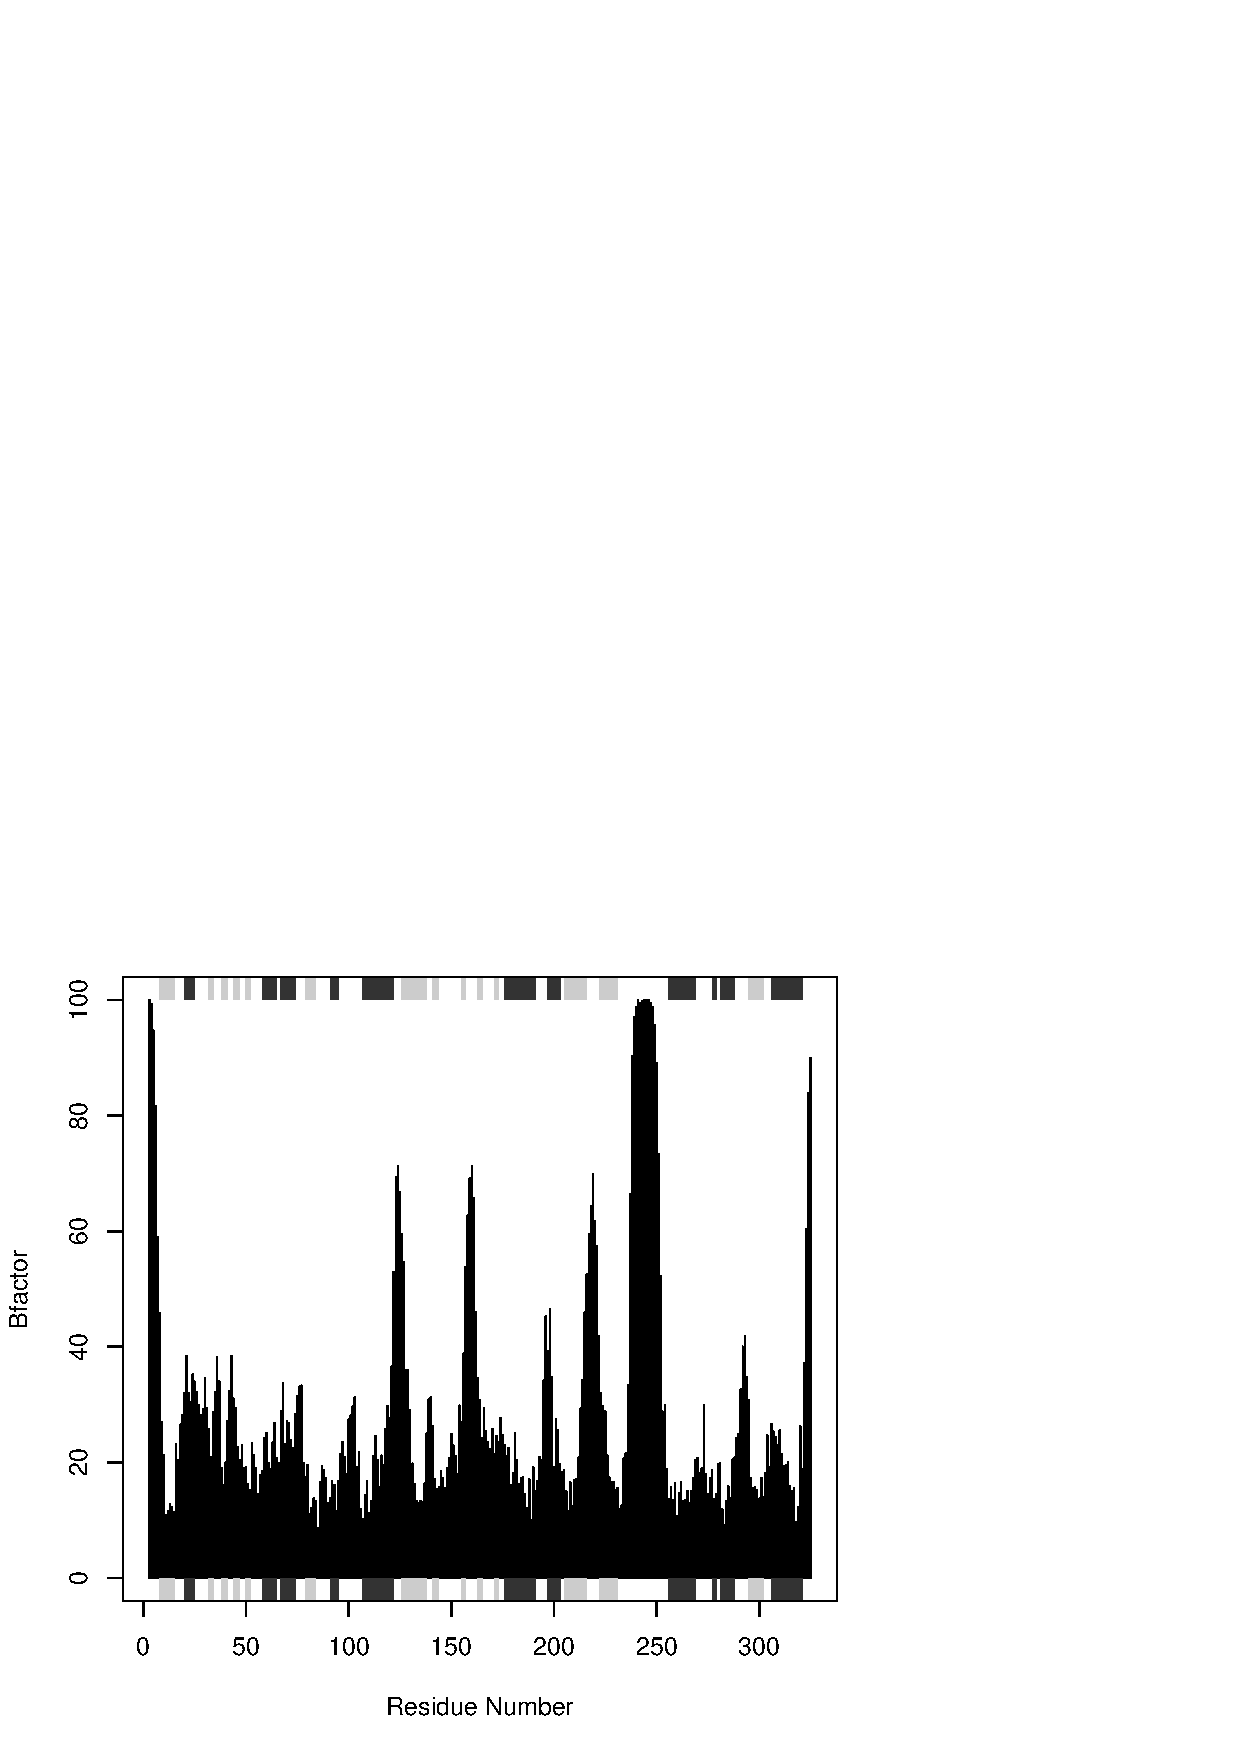
\includegraphics{figs/fig-005}
The returned \texttt{inds} object is a list containing atom and xyz numeric indices (in this case corresponding to all alpha Carbon atoms). In the above example we use these indices to plot residue number vs B-factor along with a basic secondary structure schematic. We will return to discuss atom selection in more detail in a subsequent section but as a further example of data access lets extract the sequence for the loop region between strand four and helix four in our \texttt{pdb} object.
\begin{Schunk}
\begin{Sinput}
> loop <- pdb$sheet$end[4]:pdb$helix$start[4]
> loop.inds <- atom.select(pdb, "///loop///CA/")
\end{Sinput}
\begin{Soutput}
      segid  chain  resno  resid  eleno  elety
Stest ""     ""     "loop" ""     ""     "CA" 
Natom "2527" "2527" "57"   "2527" "2527" "323"
 *  Selected a total of: 8 intersecting atoms  *
\end{Soutput}
\begin{Sinput}
> pdb$atom[loop.inds$atom, "resid"]
\end{Sinput}
\begin{Soutput}
[1] "TYR" "GLY" "GLN" "THR" "SER" "SER" "GLY" "LYS"
\end{Soutput}
\begin{Sinput}
> aa321(pdb$atom[loop.inds$atom, "resid"])
\end{Sinput}
\begin{Soutput}
[1] "Y" "G" "Q" "T" "S" "S" "G" "K"
\end{Soutput}
\end{Schunk}
In the above example the residue numbers in the \texttt{sheet} and \texttt{helix} components of \texttt{pdb} are accessed and used in a subsequent atom selection. The \texttt{aa321()} function converts between three-letter and one-letter IUPAC aminoacid codes.

Note that \texttt{pdb} object can be passed to other bio3d functions without the need for atom selection, including \texttt{torsion.pdb()}, \texttt{convert.pdb()}, \texttt{dssp()} and the distance matrix function \texttt{dm()}:
% <<fig=TRUE>>=
% d <- dm(pdb)
% plot(d, xlab="Residue Index", ylab="Residue Index")
% @

\subsection{Example Data}
A number of example datasets are included with the bio3d package. The main purpose of including this data (which may be generated by the user by following the extended examples documented within the various bio3d functions) is to allow users to more quickly appreciate the capabilities of functions that would otherwise require data input and processing before execution.


\subsubsection{The Kinesin Molecular Motor}
For the worked examples in the current document we will utilize the included kinesin dataset.  A related dataset formed the basis of the work described in \citep{grant07}.  Briefly, kinesins are molecular motor proteins responsible for the ATP dependent transport of cellular cargo along microtubules.  Kinesin family members have been found in all eukaryotic organisms, where they contribute to the transport of molecules and organelles, organisation and maintenance of the cytoskeleton, and the segregation of genetic material during mitosis and meiosis. 

The defining attribute of kinesin family members is the possession of one or more globular motor domains. These $\sim$350 residue domains are responsible for ATP hydrolysis, microtubule binding and force production. The current dataset consists of kinesin motor domain sequence and structural data and can be loaded with the command \texttt{data(kinesin)}:

\begin{Schunk}
\begin{Sinput}
> data(kinesin)
> attach(kinesin)
\end{Sinput}
\begin{Soutput}
	The following object(s) are masked _by_ .GlobalEnv :

	 aln sse xyz 


	The following object(s) are masked from kinesin ( position 3 ) :

	 aln core pc.xray pdbs sse xyz 


	The following object(s) are masked from kinesin ( position 4 ) :

	 aln core pc.xray pdbs sse xyz 
\end{Soutput}
\end{Schunk}
\paragraph{Note:}The kinesin dataset can be assembled with the \texttt{read.fasta()} and \texttt{read.fasta.pdb()} commands bellow, which read a kinesin alignment and corresponding PDB structure files:

\begin{Schunk}
\begin{Sinput}
> aln.file <- system.file("examples/kinesin_xray.fa", package = "bio3d")
> pdb.path <- system.file("examples/", package = "bio3d")
> aln <- read.fasta(aln.file)
> pdbs <- read.fasta.pdb(aln, pdb.path = pdb.path, pdbext = ".ent")
\end{Sinput}
\end{Schunk}



%%%%%%%%%%%%%%%%%%%%%%%%%%%%%%%%%%%%%%%%%%%%%%%%%%%%%%%
% --------------
% Second section 
% --------------

\section{Sample Applications of bio3d}
Comparing multiple structures of homologous proteins and carefully analysing large multiple sequence alignments can help identify patterns of sequence and structural conservation and highlight conserved interactions that are crucial for protein stability and function \citep{grant07}.  Bio3d and R provide a useful framework for such sudies and facilate the integration of sequence, structure and dynamics data in the analysis of protein evolution.


\subsection{Comparative Structural Analysis}
The detailed comparison of homologous protein structures can be used to infer pathways for evolutionary adaptation and, at closer evolutionary distances, mechanisms for conformational change. The bio3d package employs refined structural superposition and principal component analysis (PCA) to examine the relationship between different conformers. 

\subsubsection{Interconformer Relationships with PCA}
Conventional structural superposition of proteins minimizes the root mean square difference between their full set of equivalent residues. However, for the current application such a superposition procedure can be inappropriate. For example, in the comparison of a multi-domain protein that has undergone a hinge-like rearrangement of its domains, standard all atom superposition would result in an underestimate of the true atomic displacement by attempting superposition over all domains (whole structure superposition). A more appropriate and insightful superposition would be anchored at the most invariant region and hence more clearly highlight the domain rearrangement (sub-structure superposition). 


\paragraph{Sub-structure Superposition:}
The \texttt{core.find()} function implements an iterated superposition procedure, where residues displaying the largest positional differences are identified and excluded at each round.  The function returns an ordered list of excluded residues, from which the user can select a subset of 'core' residues upon which superposition can be based.

\begin{Schunk}
\begin{Sinput}
> core <- core.find(pdbs)
\end{Sinput}
\end{Schunk}
There are \texttt{plot.core()} and \texttt{print.core()} functions available for further examining the output of \texttt{core.find()}.
\begin{center}
\begin{Schunk}
\begin{Sinput}
> col = rep("black", length(core$volume))
> col[core$volume < 2] = "pink"
> col[core$volume < 1] = "red"
> plot(core, col = col)
\end{Sinput}
\end{Schunk}
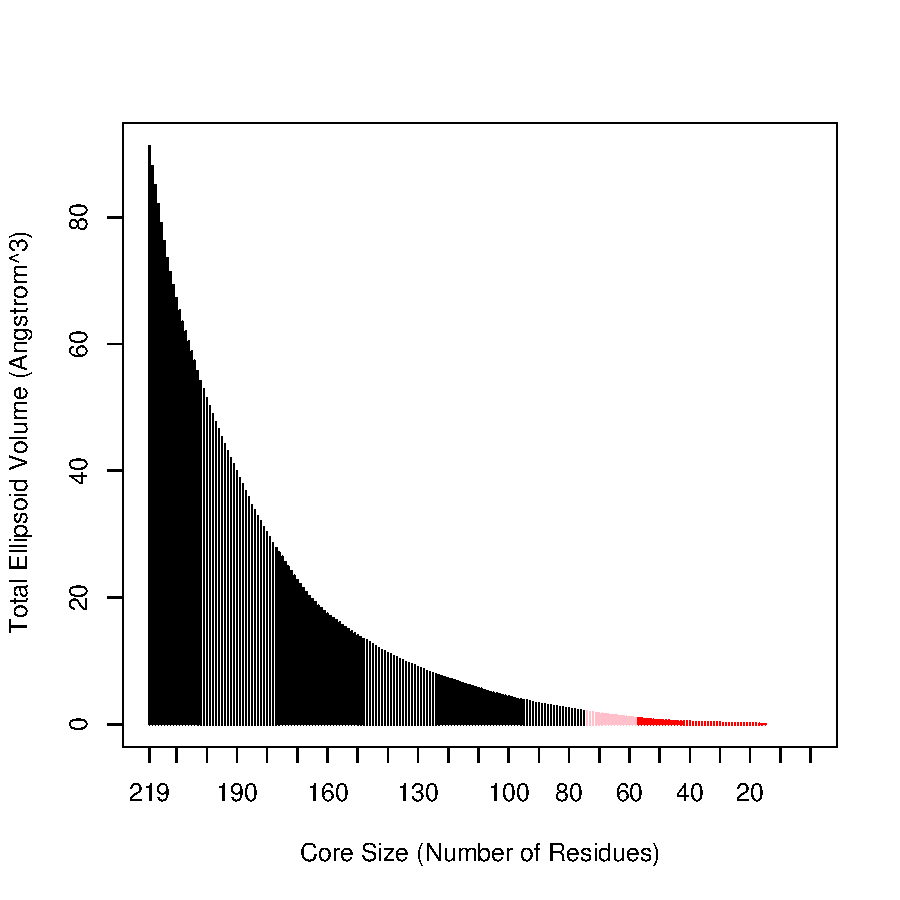
\includegraphics{figs/fig-010}
% \caption{Figure 1. core.find plot.}
\end{center}
The \texttt{print.core()} function also returns \texttt{atom} and \texttt{xyz} indices.  Below we select a subset of positions with a cumulative ellipsoid volume of less than 0.5 \AA $^3$ and use the returned indices to write a quick PDB file for viewing in a molecular graphics program (Figure 2).  
\begin{Schunk}
\begin{Sinput}
> inds <- print(core, vol = 0.5)
\end{Sinput}
\begin{Soutput}
# 44 positions (cumulative volume <= 0.5 Angstrom^3) 
  start end length
1    10  15      6
2    51  52      2
3    80  94     15
4   207 209      3
5   228 232      5
6   235 235      1
7   297 302      6
8   311 316      6
\end{Soutput}
\begin{Sinput}
> write.pdb(xyz = pdbs$xyz[1, inds$xyz], resno = pdbs$resno[1, 
+     inds$atom], file = "quick_core.pdb")
\end{Sinput}
\end{Schunk}

\begin{center}
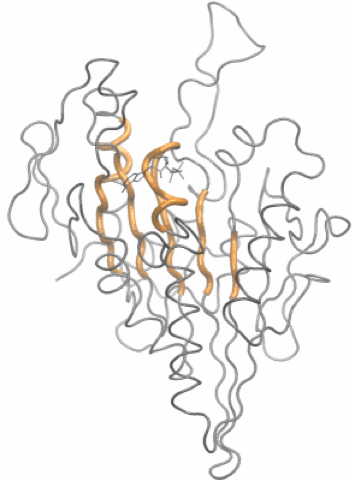
\includegraphics[width=60mm]{figs/core.png}
\end{center}
We can now superpose all structures on the selected core indices with the \texttt{fit.xyz()} function.
\begin{Schunk}
\begin{Sinput}
> xyz <- fit.xyz(fixed = pdbs$xyz[1, ], mobile = pdbs, fixed.inds = inds$xyz, 
+     mobile.inds = inds$xyz)
\end{Sinput}
\end{Schunk}
The above command performs the actual superposition and stores the new coordinats in the matrix object \texttt{xyz}.  By providing several extra arguments to \texttt{fit.xyz()} a directory, here named \texttt{fitlsq}, containing superposed structures can be produced.
\begin{Schunk}
\begin{Sinput}
> xyz <- fit.xyz(fixed = pdbs$xyz[1, ], mobile = pdbs, fixed.inds = inds$xyz, 
+     mobile.inds = inds$xyz, pdb.path = system.file("examples/", 
+         package = "bio3d"), pdbext = ".ent", outpath = "fitlsq/", 
+     full.pdbs = TRUE)
\end{Sinput}
\begin{Soutput}
  HEADER    SCOP/ASTRAL domain d1bg2__ [32189]      03-FEB-05   0000 
  HEADER    SCOP/ASTRAL domain d1mkja_ [79239]      03-FEB-05   0000 
  HEADER    SCOP/ASTRAL domain d2kin.1 [32190]      03-FEB-05   0000 
   PDB has ALT records, taking A only, rm.alt=TRUE
  HEADER    SCOP/ASTRAL domain d3kin.1 [32191]      03-FEB-05   0000 
  HEADER    SCOP/ASTRAL domain d3kin.2 [32192]      03-FEB-05   0000 
  HEADER    SCOP/ASTRAL domain d1v8ka_ [100510]     07-FEB-05   0000 
  HEADER    SCOP/ASTRAL domain d1v8ja_ [100509]     07-FEB-05   0000 
  HEADER    SCOP/ASTRAL domain d1goja_ [65419]      03-FEB-05   0000 
  HEADER    SCOP/ASTRAL domain d1ry6a_ [98090]      03-FEB-05   0000 
  HEADER    SCOP/ASTRAL domain d1sdma_ [105438]     28-JUL-05   0000 
  HEADER    SCOP/ASTRAL domain d1vfva_ [108592]     28-JUL-05   0000 
  HEADER    SCOP/ASTRAL domain d1i6ia_ [61844]      03-FEB-05   0000 
   PDB has ALT records, taking A only, rm.alt=TRUE
  HEADER    SCOP/ASTRAL domain d1i5sa_ [61822]      03-FEB-05   0000 
   PDB has ALT records, taking A only, rm.alt=TRUE
  HEADER    SCOP/ASTRAL domain d1vfza_ [108595]     28-JUL-05   0000 
  HEADER    SCOP/ASTRAL domain d1vfwa_ [108593]     28-JUL-05   0000 
  HEADER    SCOP/ASTRAL domain d1vfxa_ [108594]     28-JUL-05   0000 
  HEADER    SCOP/ASTRAL domain d1q0ba_ [95502]      03-FEB-05   0000 
  HEADER    SCOP/ASTRAL domain d1q0bb_ [95503]      03-FEB-05   0000 
  HEADER    SCOP/ASTRAL domain d1ii6a_ [62413]      03-FEB-05   0000 
  HEADER    SCOP/ASTRAL domain d1ii6b_ [62414]      03-FEB-05   0000 
  HEADER    SCOP/ASTRAL domain d2ncda_ [32193]      03-FEB-05   0000 
  HEADER    SCOP/ASTRAL domain d1cz7a_ [32194]      03-FEB-05   0000 
  HEADER    SCOP/ASTRAL domain d1cz7b_ [32195]      03-FEB-05   0000 
  HEADER    SCOP/ASTRAL domain d1cz7c_ [32196]      03-FEB-05   0000 
  HEADER    SCOP/ASTRAL domain d1cz7d_ [32197]      03-FEB-05   0000 
  HEADER    SCOP/ASTRAL domain d1n6ma_ [91688]      03-FEB-05   0000 
  HEADER    SCOP/ASTRAL domain d1n6mb_ [91689]      03-FEB-05   0000 
  HEADER    SCOP/ASTRAL domain d1f9va_ [59745]      03-FEB-05   0000 
  HEADER    SCOP/ASTRAL domain d1f9ta_ [59743]      03-FEB-05   0000 
  HEADER    SCOP/ASTRAL domain d1f9ua_ [59744]      03-FEB-05   0000 
  HEADER    SCOP/ASTRAL domain d3kar__ [32198]      03-FEB-05   0000 
  HEADER    SCOP/ASTRAL domain d1f9wa_ [59746]      03-FEB-05   0000 
  HEADER    SCOP/ASTRAL domain d1f9wb_ [59747]      03-FEB-05   0000 
\end{Soutput}
\end{Schunk}
These can then be viewed in your favoriate molecular graphics program (Figure 3).

\begin{center}
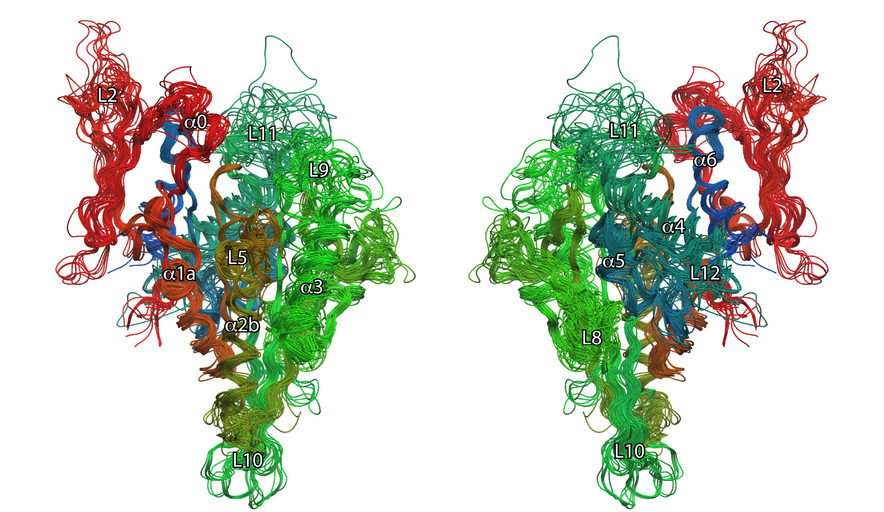
\includegraphics[width=120mm]{figs/fit.png}
\end{center}

\paragraph{Principal Component Analysis:}
Following core identification and subsequent superposition, PCA can be employed to examine the relationship between different structures based on their equivalent residues. The application of PCA to both distributions of experimental structures and molecular dynamics trajectories, along with its ability to provide considerable insight into the nature of conformational differences has been discussed previously (see \citet{grant07} and references therein).  

Briefly, the resulting principal components (orthogonal eigenvectors) describe the axes of maximal variance of the distribution of structures. Projection of the distribution onto the subspace defined by the largest principal components results in a lower dimensional representation of the structural dataset. The percentage of the total mean square displacement (or variance) of atom positional fluctuations captured in each dimension is characterized by their corresponding eigenvalue. Experience suggests that 3--5 dimensions are often sufficient to capture over 70 percent of the total variance in a given family of structures. Thus, a handful of principal components are sufficient to provide a useful description while still retaining most of the variance in the original distribution \citet{grant06}. 


\begin{Schunk}
\begin{Sinput}
> cut.seqs <- which(pdbs$id %in% c("d1n6mb_", "d1ry6a_"))
> gaps.res <- gap.inspect(pdbs$ali[-cut.seqs, ])
> gaps.pos <- gap.inspect(pdbs$xyz[-cut.seqs, ])
> pc.xray <- pca.xyz(xyz[-cut.seqs, gaps.pos$f.inds])
\end{Sinput}
\end{Schunk}
The above sequence of commands returns the indices of two structures and the indices for gap containing positions, both of which we exclude from subsequent PCA with the \texttt{pca.xyz()} command. A quick overview of the results of \texttt{pca.xyz()} can be obtained by calling \texttt{plot.pca()}

\begin{center}
\begin{Schunk}
\begin{Sinput}
> plot(pc.xray)
\end{Sinput}
\end{Schunk}
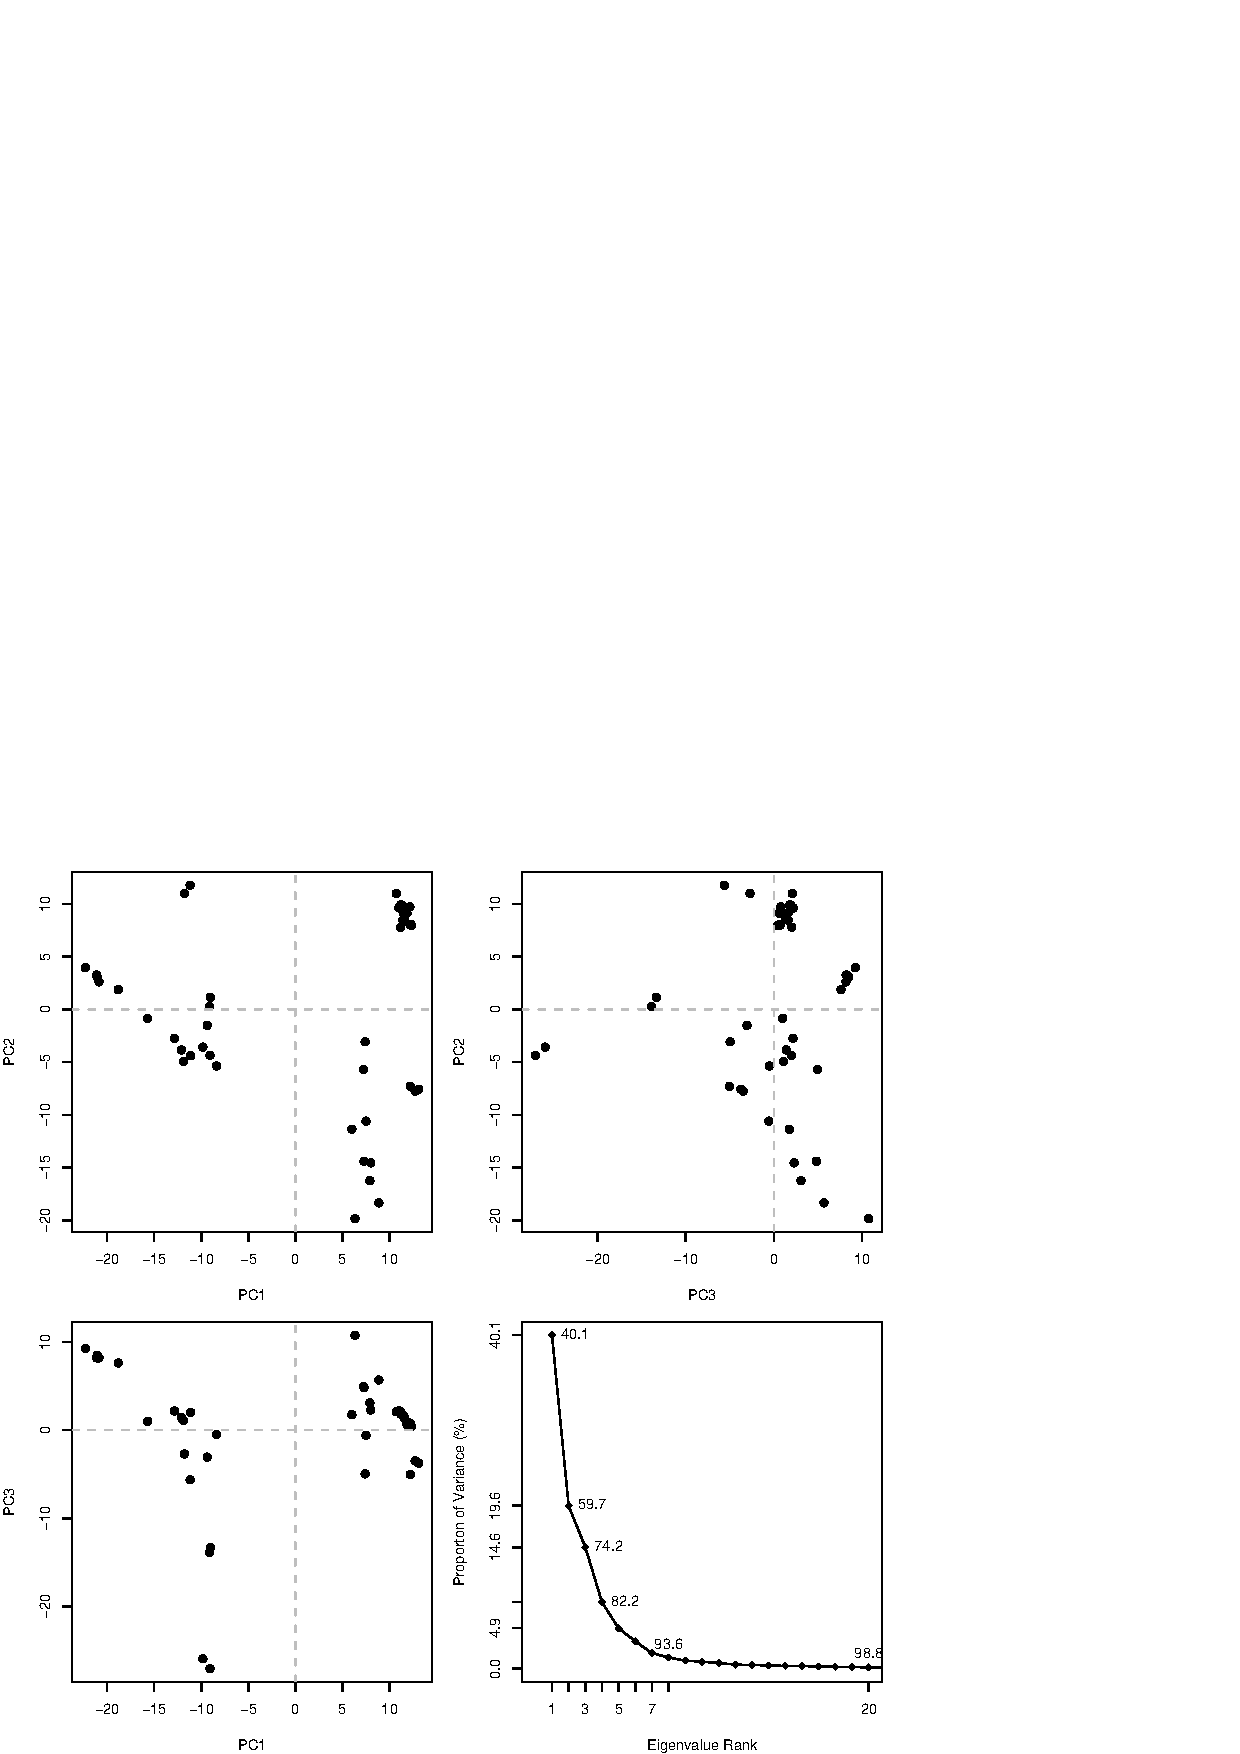
\includegraphics{figs/fig-016}
\end{center}

and calling  \texttt{plot.bio3d()} to examine the contribution of each residue to the first three principal components.

\begin{center}
\begin{Schunk}
\begin{Sinput}
> res.ref <- which(!is.gap(pdbs$ali["d1bg2__", ]))
> res.ind <- which(res.ref %in% gaps.res$f.ind)
> par(mfrow = c(3, 1), cex = 0.6, mar = c(3, 4, 1, 1))
> plot.bio3d(res.ind, pc.xray$au[, 1], sse = sse, ylab = "PC1 (A)")
> plot.bio3d(res.ind, pc.xray$au[, 2], sse = sse, ylab = "PC2 (A)")
> plot.bio3d(res.ind, pc.xray$au[, 3], sse = sse, ylab = "PC3 (A)")
\end{Sinput}
\end{Schunk}
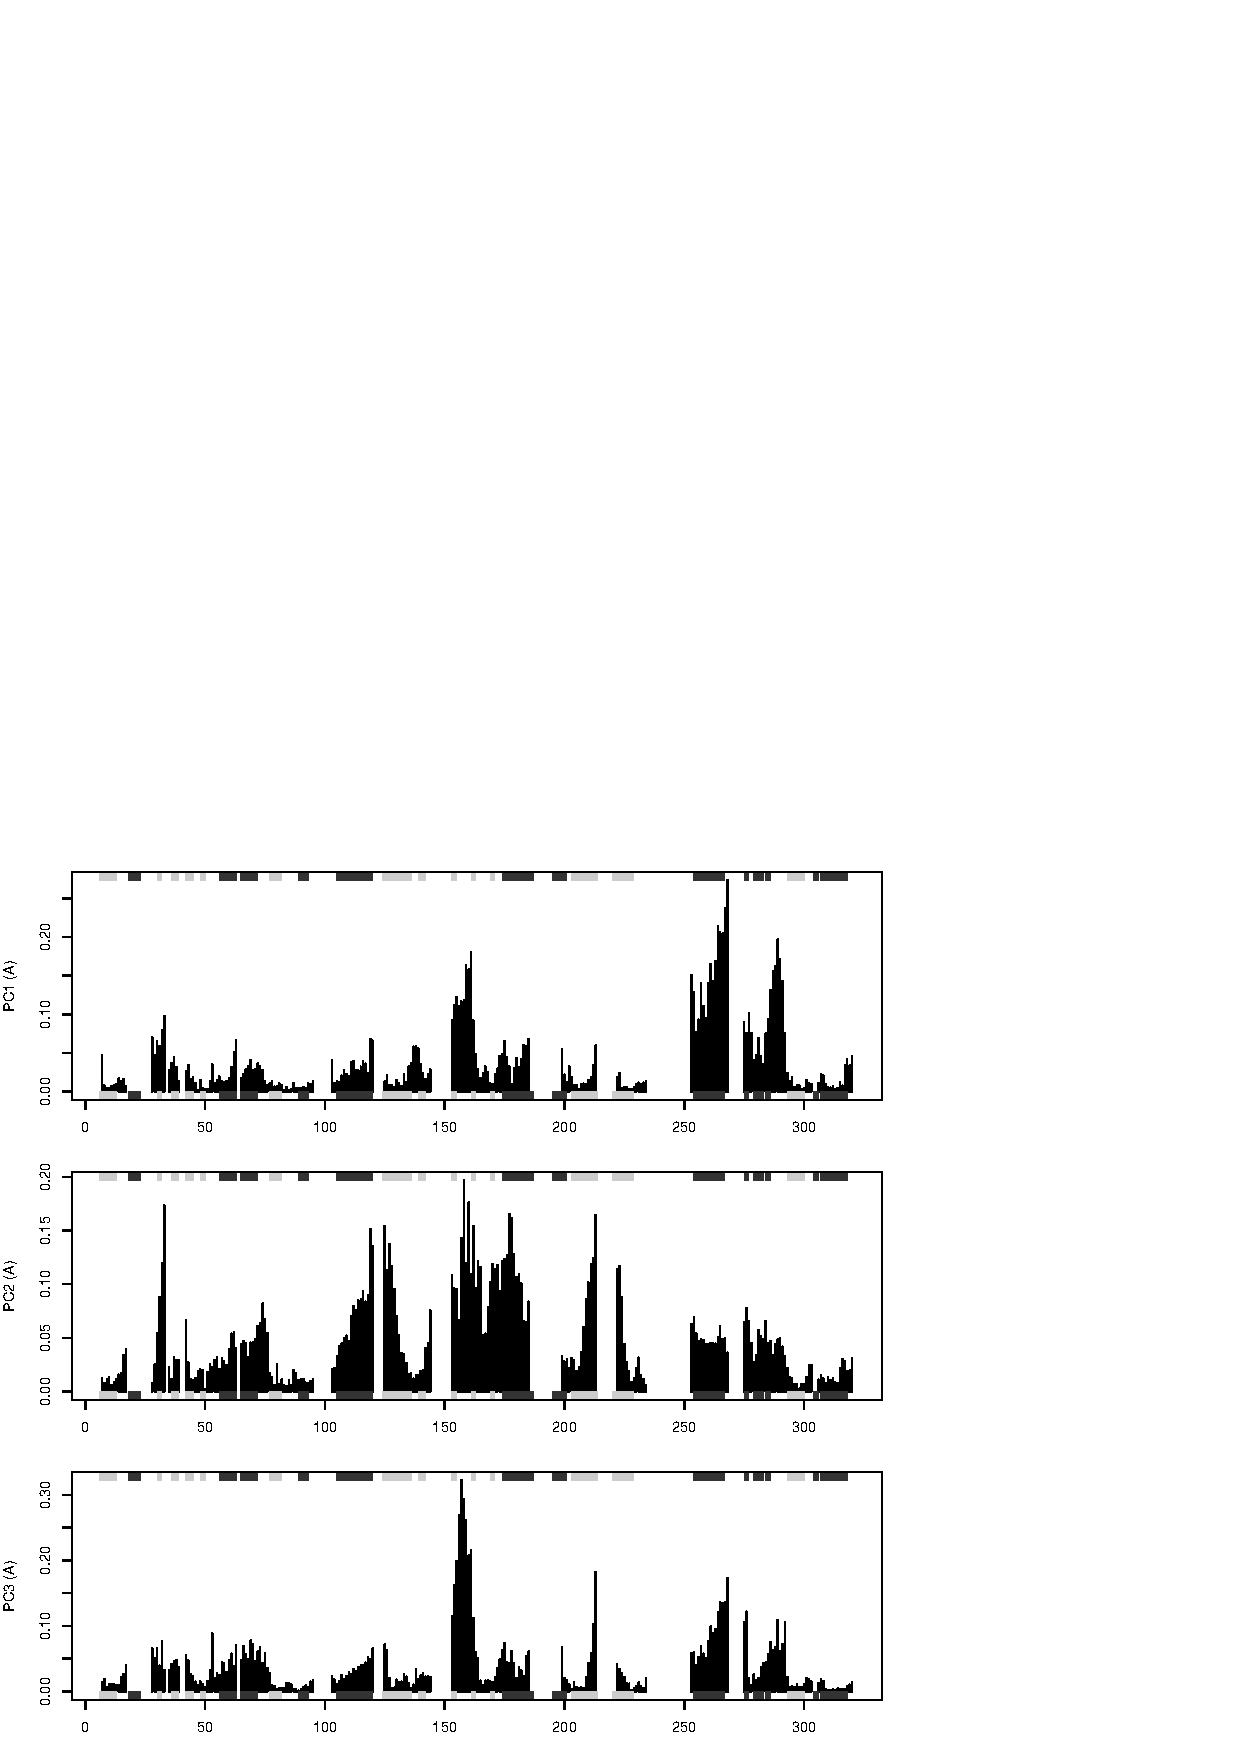
\includegraphics{figs/fig-017}
\end{center}

The plots in figures 4 and 5 display the relationships between different conformers, highlight positions responsible for the major differences between structures and enable the interpretation and characterization of multiple interconformer relationships.


\paragraph{Structure Interpolation:}
To further aid interpretation, a PDB format trajectory can be produced that interpolates between the most dissimilar structures in the distribution along a given principal cmponent.  This involves dividing the difference between the conformers into a number of evenly spaced steps along the principal components, forming the frames of the trajectory. Such trajectories can be directly visualized in a molecular graphics program, such as VMD \citep{vmd}. Furthermore, the interpolated structures can be analyzed for possible domain and shear movements with the DynDom package \citep{dyndom}, or used as initial seed structures for more advanced reaction path refinement methods such as Conjugate Peak Refinement \citep{cpr}.

\begin{Schunk}
\begin{Sinput}
> a <- mktrj.pca(pc.xray, pc = 1, file = "pc1.pdb", resno = pdbs$resno[1, 
+     gaps.res$f.inds], resid = aa123(pdbs$ali[1, gaps.res$f.inds]))
\end{Sinput}
\end{Schunk}

\begin{center}
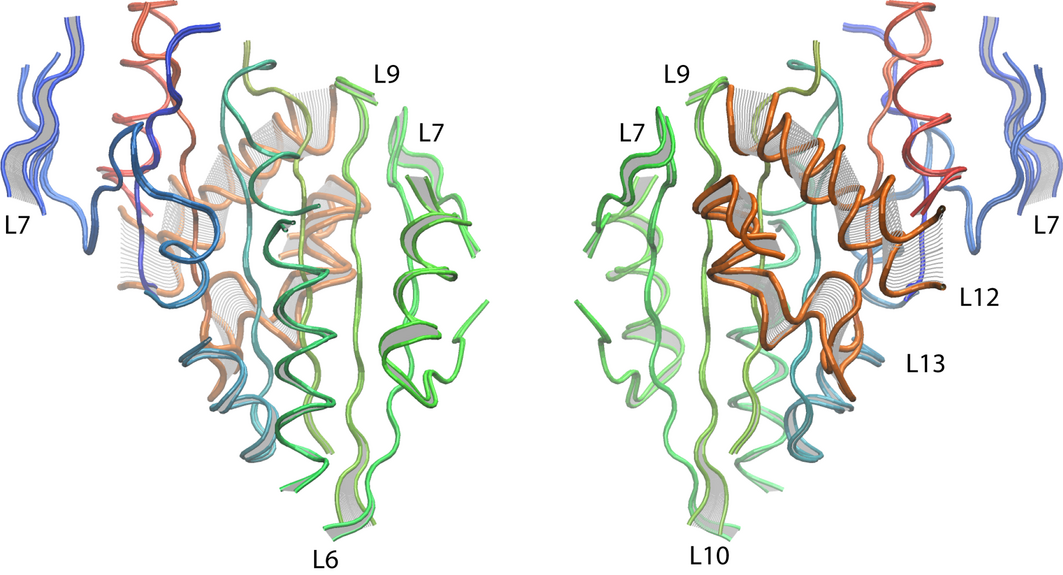
\includegraphics[width=100mm]{figs/pca.png}
\end{center}

\paragraph{Conformer Clustering in PC space}
Clustering of structures in the PC1-3 planes

\begin{center}
\begin{Schunk}
\begin{Sinput}
> plot(hclust(dist(pc.xray$z[, 1:3])), labels = substr(pdbs$id[-cut.seqs], 
+     2, 10), main = "PC1-3")
\end{Sinput}
\end{Schunk}
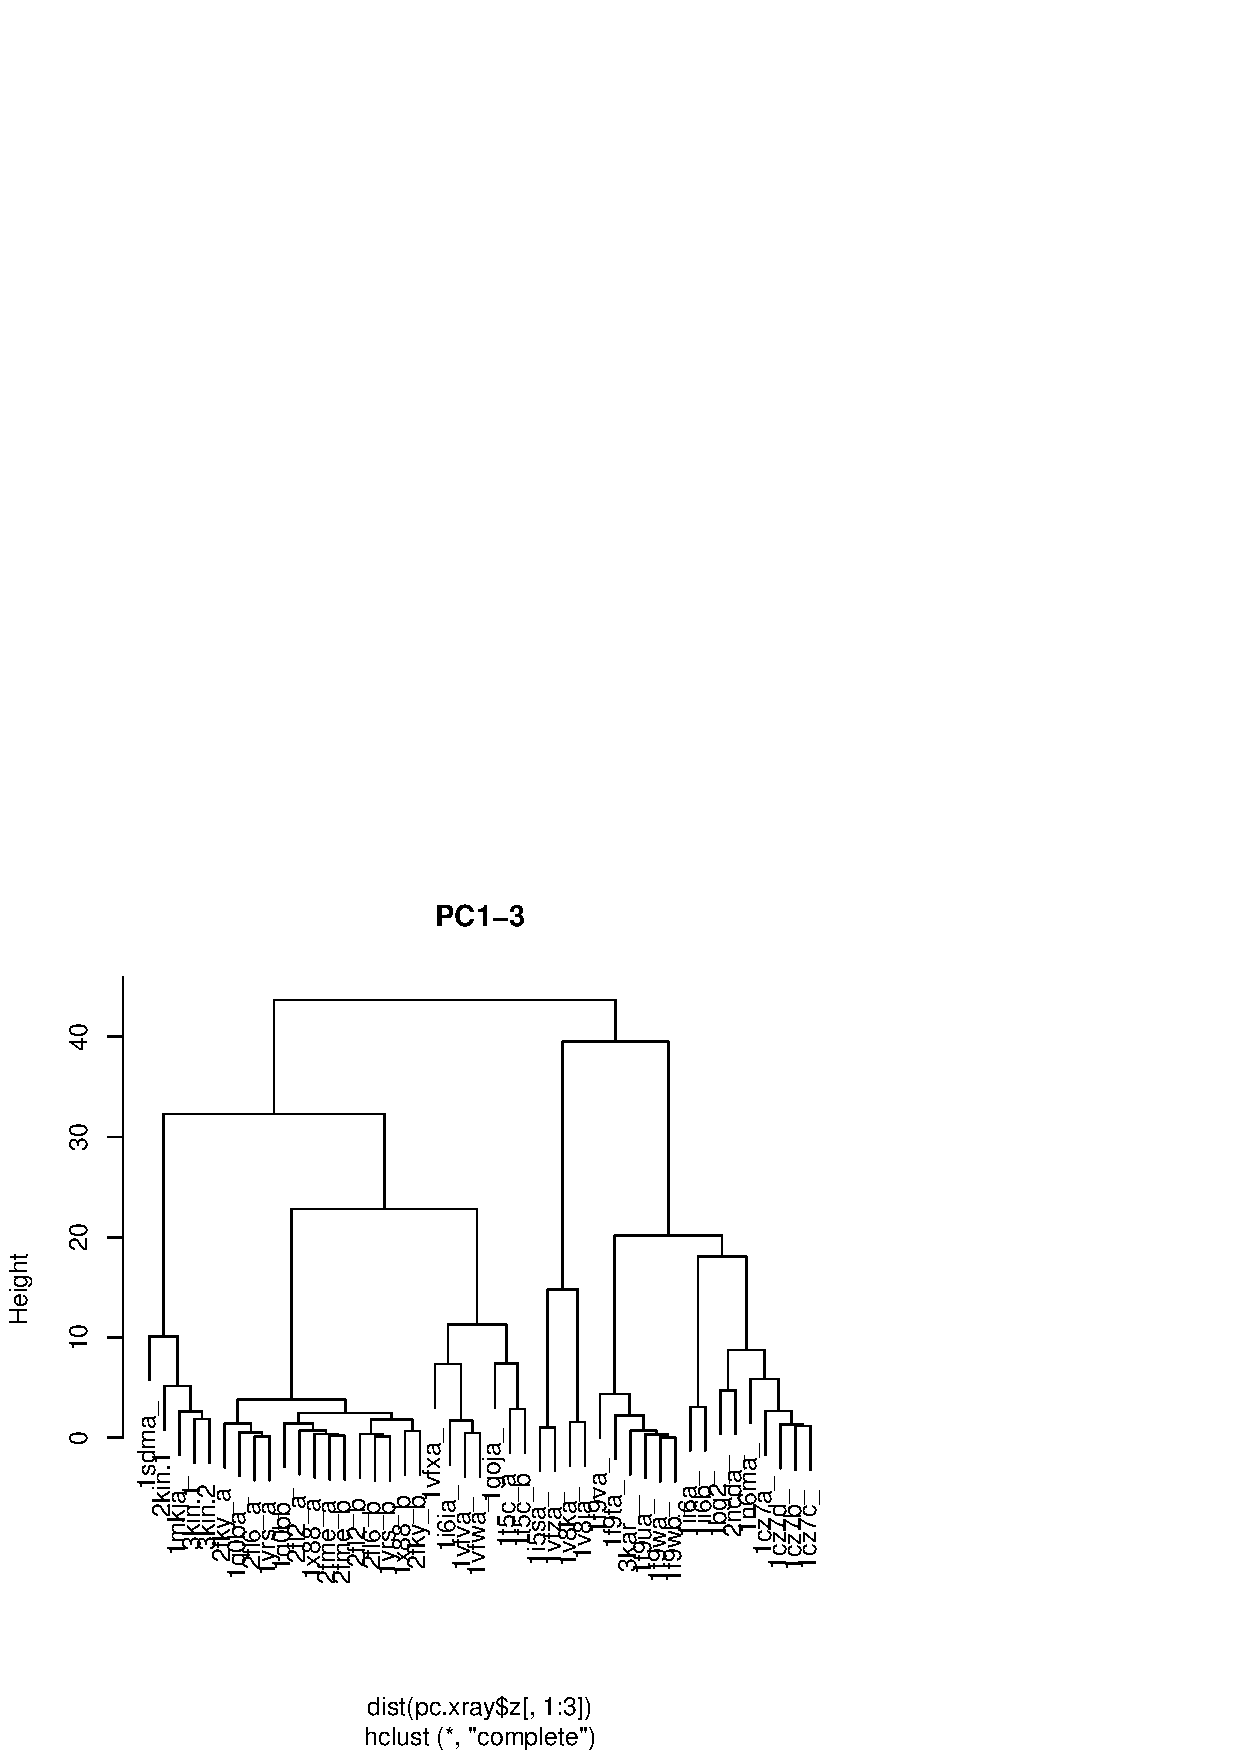
\includegraphics{figs/fig-019}
\end{center}




%%%%%%%%%%%%%%%%%%%%%%%%%%%%%%%%%%%%%%%%%%%%%%%%%%%%%%%
% Third section %

\subsubsection{Further examples}
Bio3d facilitates the analysis of various structural properties, such as root mean-square deviation (RMSD), root mean-square fluctuation (RMSF), secondary structure, dihedral angles, difference distance matrices etc. The current section provides a brief exposure to using bio3d in this vein. 

\subsection{Finding available sets of similar structures}
First lets examine one way in which we can use bio3d to find sets of similar structures. To collect available kinesin crystal structures we first use BLAST to query the PDB to find similar sequences (and hence structures) to our chosen representative (PDB c ode 1BG2).

\begin{Schunk}
\begin{Sinput}
> pdb <- read.pdb(get.pdb("1bg2", URLonly = TRUE))
\end{Sinput}
\begin{Soutput}
  HEADER    MOTOR PROTEIN                           04-JUN-98   1BG2               
\end{Soutput}
\begin{Sinput}
> seq <- seq.pdb(pdb)
\end{Sinput}
\begin{Soutput}
      segid  chain  resno  resid  eleno  elety
Stest ""     ""     ""     ""     ""     "CA" 
Natom "2527" "2527" "2527" "2527" "2527" "323"
 *  Selected a total of: 323 intersecting atoms  *
\end{Soutput}
\begin{Sinput}
> blast <- blast.pdb(seq)
\end{Sinput}
\begin{Soutput}
 Searching ... please wait (updates every 5 seconds) RID = 8VUJ6WWJ012 
 .
 Reporting 158 hits
\end{Soutput}
\end{Schunk}
Examining the alignment scores and their associated E-values (with the function \texttt{plot.blast()}) indicates a sensible normalized score (-log(E-Value)) cutoff of ~50 bits.


\begin{figure}[hbtp]
\begin{center}
\begin{Schunk}
\begin{Sinput}
> hits <- plot.blast(blast, cutoff = 50)
> head(hits)
\end{Sinput}
\begin{Soutput}
  pdb.id   gi.id      
1 "1MKJ_A" "24987772" 
2 "1BG2_A" "157830287"
3 "2P4N_K" "193885175"
4 "2KIN_A" "3114353"  
5 "3KIN_A" "3891776"  
6 "3KIN_C" "3891778"  
\end{Soutput}
\end{Schunk}
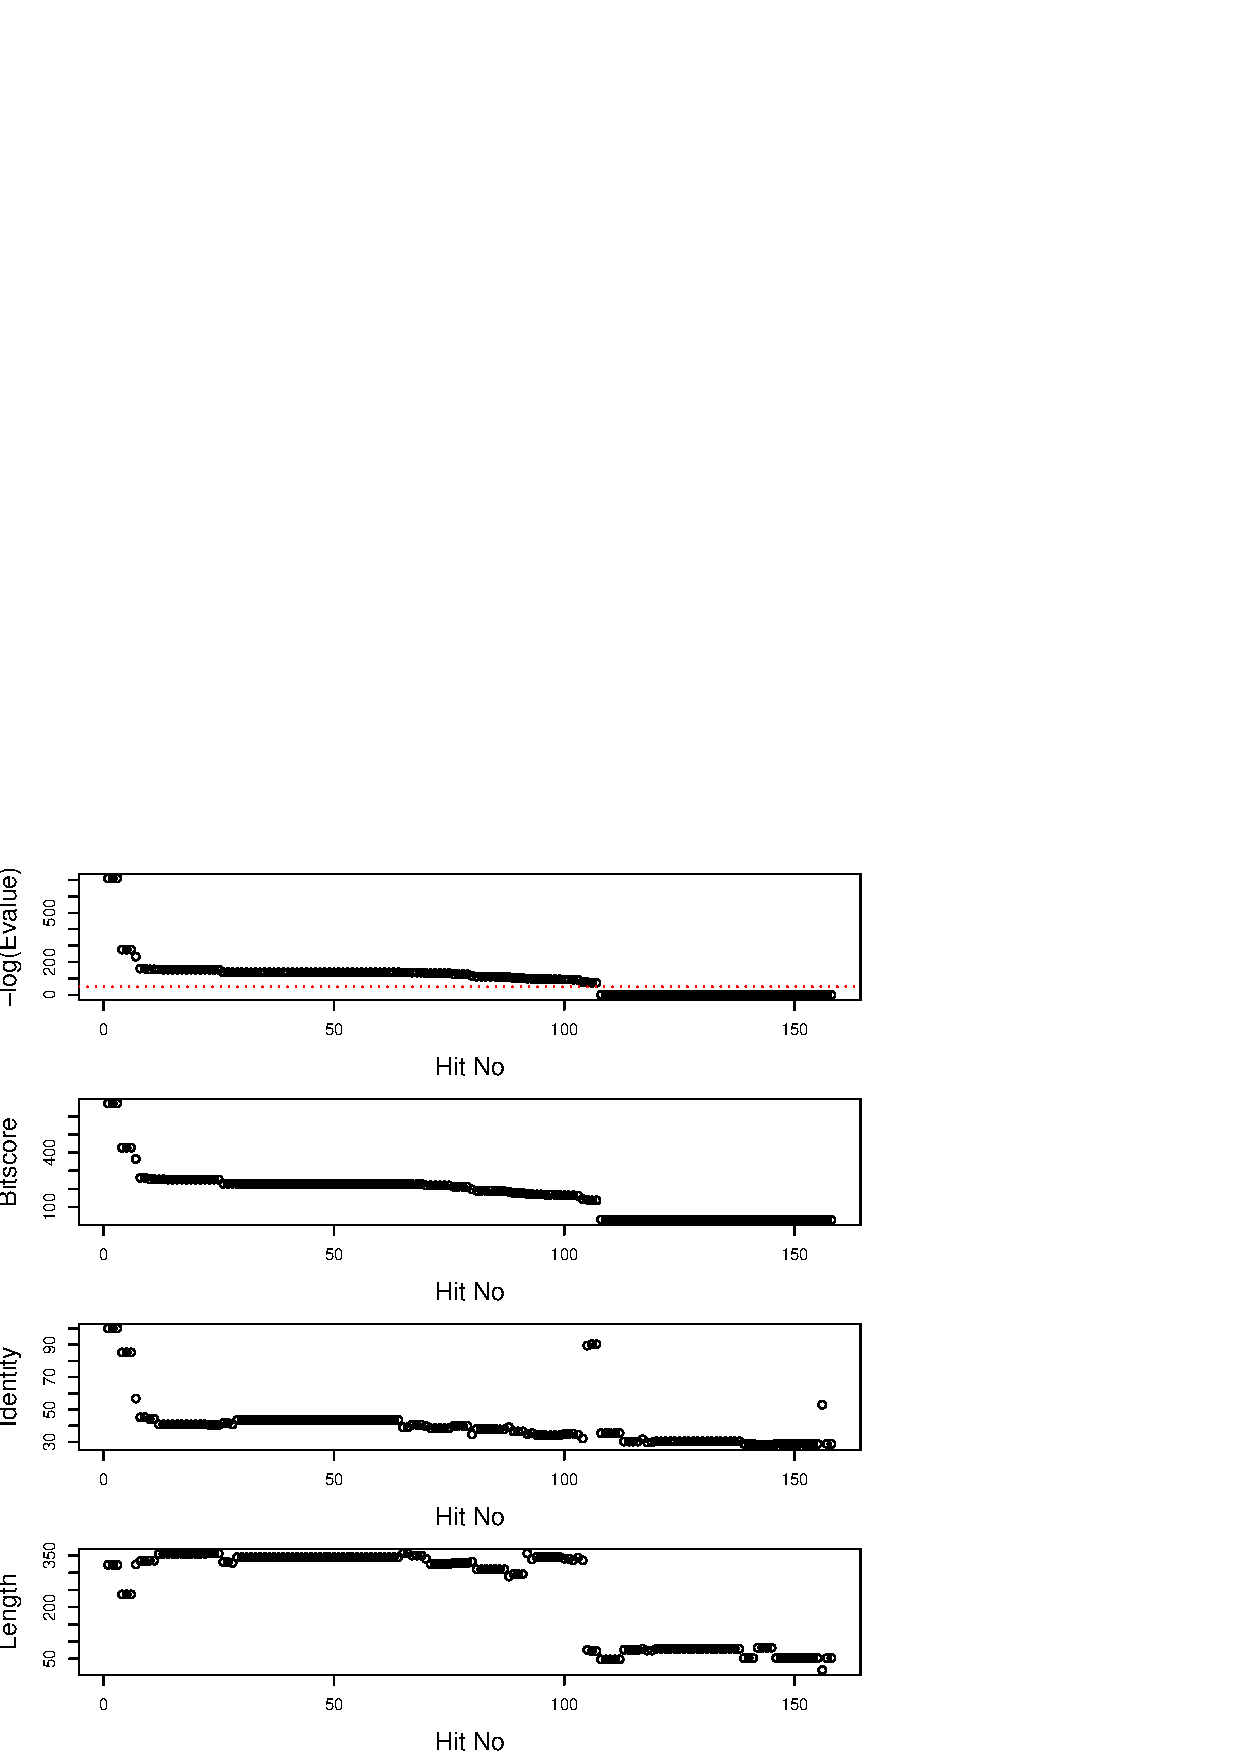
\includegraphics{figs/fig-blasthits}
\label{fig:blast}
\end{center}
\end{figure}

\paragraph{Unfinished section of draft!}

\paragraph{Atom selection:} 
Bio3d provides an atom selection function (\texttt{atom.select()}) that returns atom and xyz indicies corresponding to the intersection of a hierarchical selection string.  Once an atom selection is made, you can query the properties of the selected atoms, such as their names, residue ids, or coordinates. In a similar fashion, you can set the values of these properties. You can also perform logical operations on atom selections, including finding the intersection or union of two or more atom selections or finding the inverse of the set.

\paragraph{Root mean square deviation (RMSD):}
RMSD is a standard measure of structural distance between coordinate sets.
\begin{Schunk}
\begin{Sinput}
> gaps.xyz <- gap.inspect(pdbs$xyz)
> rd.raw <- rmsd(pdbs$xyz[, gaps.xyz$f.inds])
> rd.fit <- rmsd(pdbs$xyz[, gaps.xyz$f.inds], fit = TRUE)
> range(rd.raw)
\end{Sinput}
\begin{Soutput}
[1]   0.000 234.692
\end{Soutput}
\begin{Sinput}
> range(rd.fit)
\end{Sinput}
\begin{Soutput}
[1] 0.000 2.447
\end{Soutput}
\end{Schunk}

\begin{center}
\begin{Schunk}
\begin{Sinput}
> rmsd.fit <- rmsd(pdbs$xyz[1, gaps.xyz$f.inds], pdbs$xyz[, gaps.xyz$f.inds], 
+     fit = TRUE)
> hist(rmsd.fit)
\end{Sinput}
\end{Schunk}
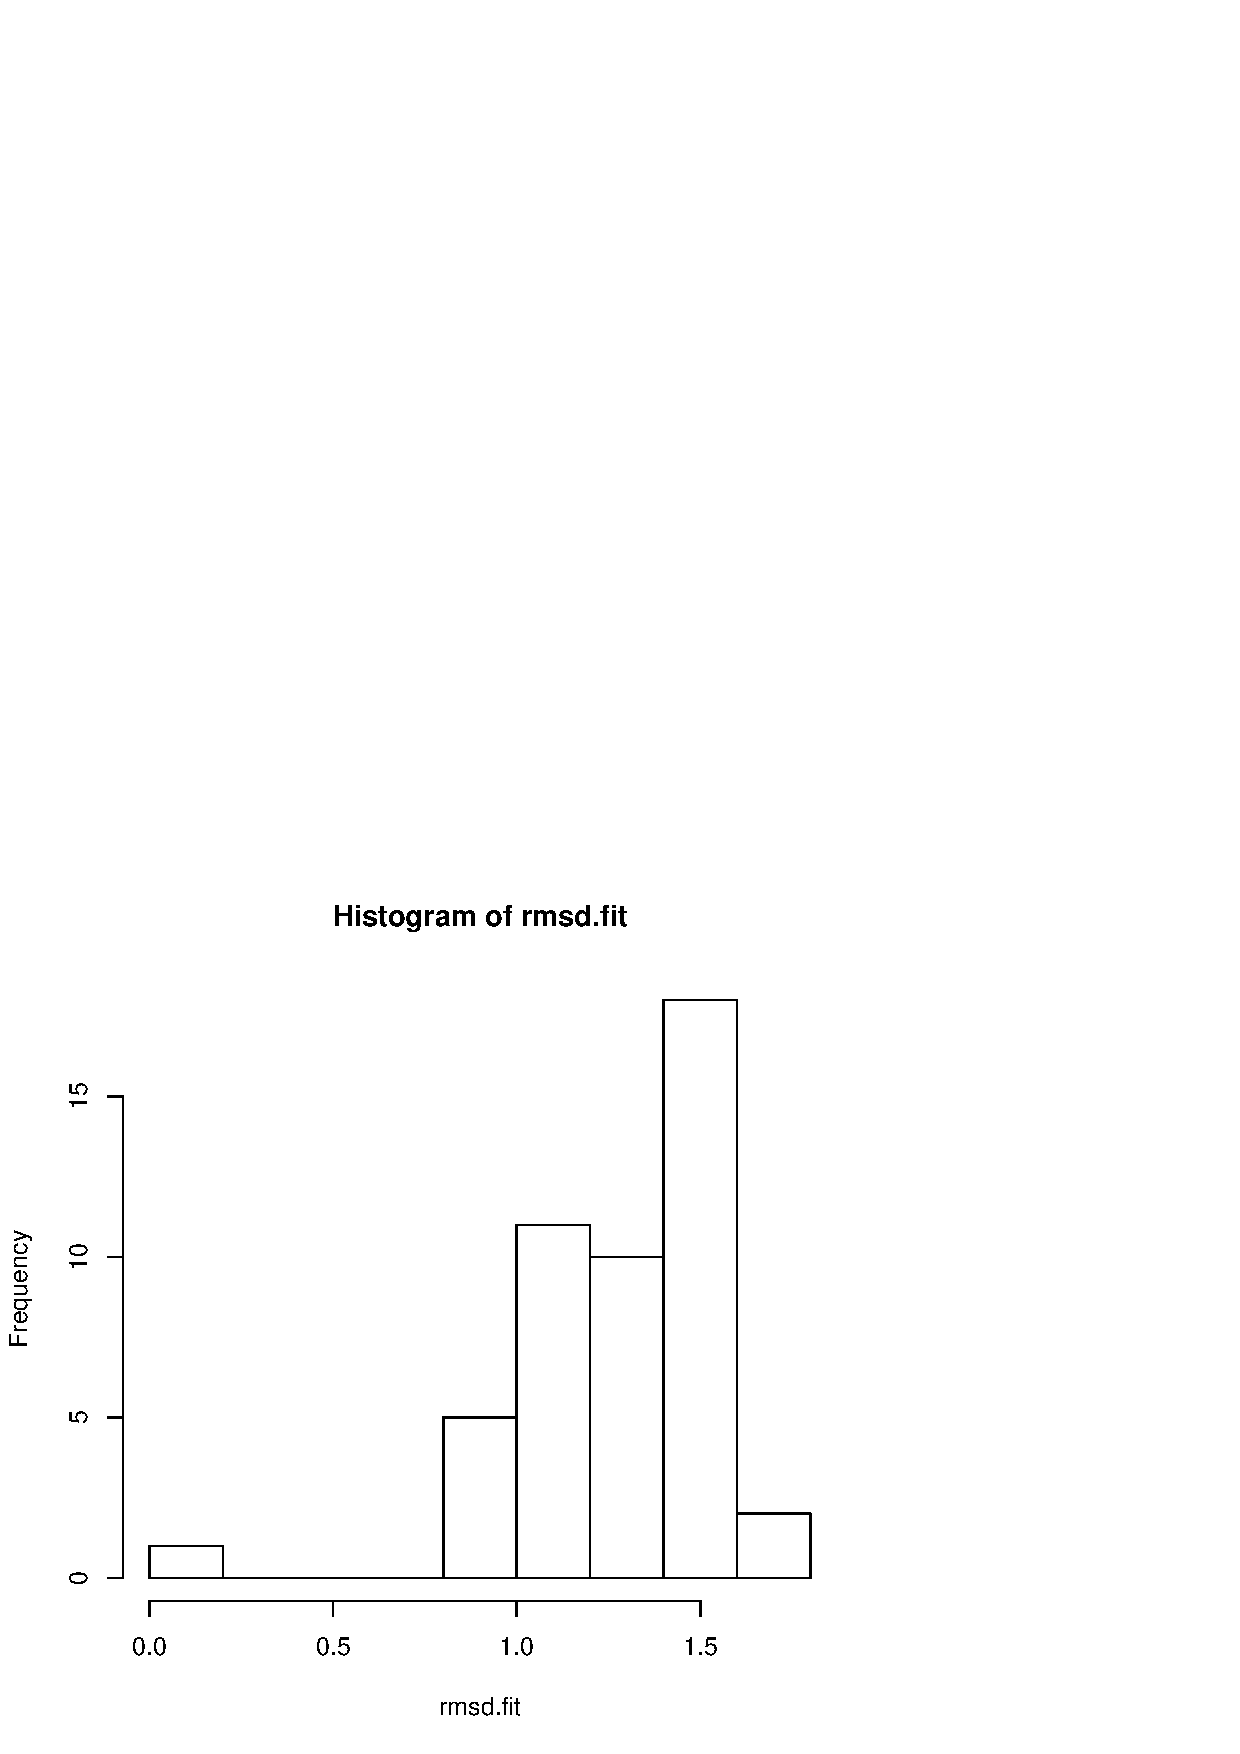
\includegraphics{figs/fig-023}
\end{center}


\paragraph{Clustering:}
Cluster with RMSD or see earler section on PCA [reference back]
\begin{center}
\begin{Schunk}
\begin{Sinput}
> plot(hclust(as.dist(rd.fit)), labels = substr(pdbs$id, 2, 10), 
+     ylab = "RMSD", xlab = "")
\end{Sinput}
\end{Schunk}
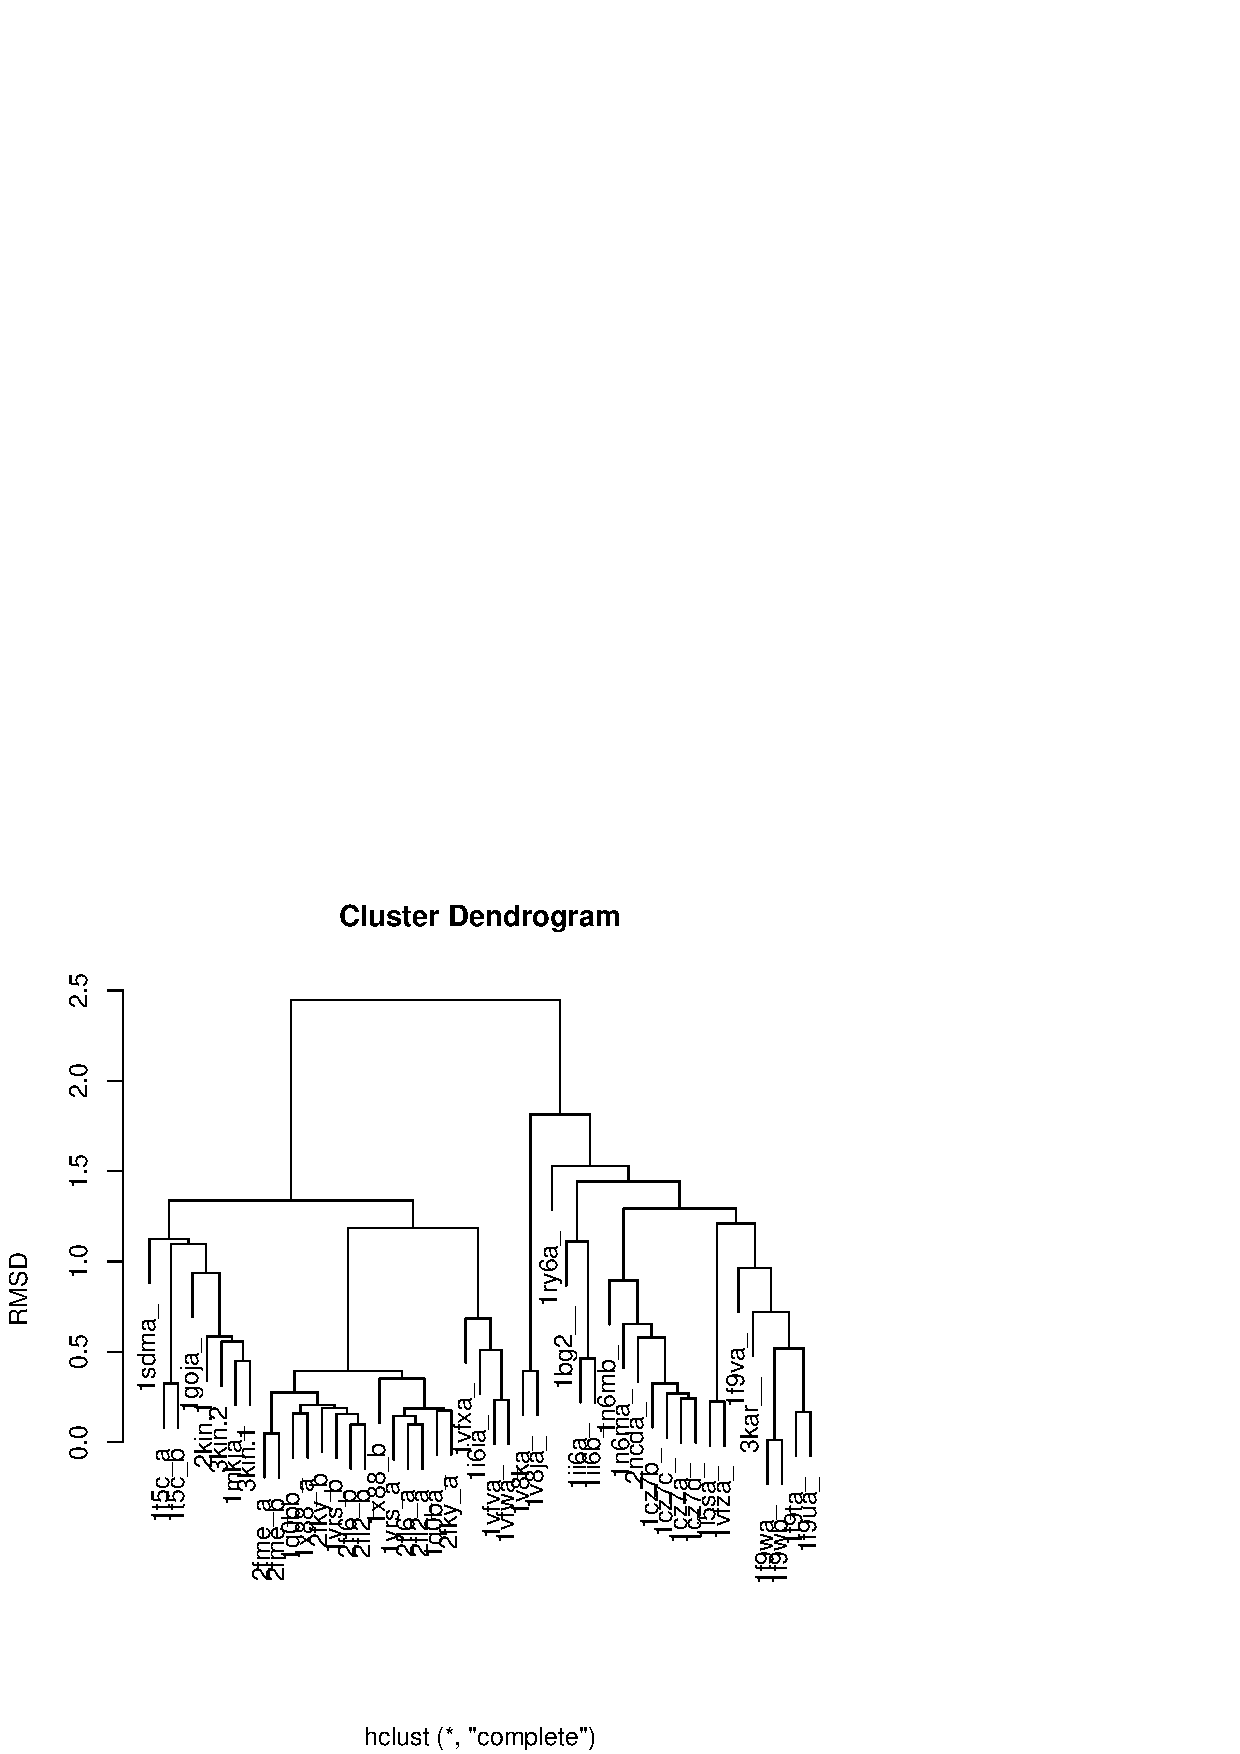
\includegraphics{figs/fig-024}
\end{center}



\paragraph{Root mean squared fluctuations (RMSF):}
RMSF is an often used measure of conformational variance.
\begin{Schunk}
\begin{Sinput}
> gaps <- is.na(pdbs$xyz[1, ])
> rf <- rmsf(xyz[, !gaps])
\end{Sinput}
\end{Schunk}

\begin{center}
\begin{Schunk}
\begin{Sinput}
> plot.bio3d(rf, sse = sse, ylab = "RMSF (A)", xlab = "Position")
\end{Sinput}
\end{Schunk}
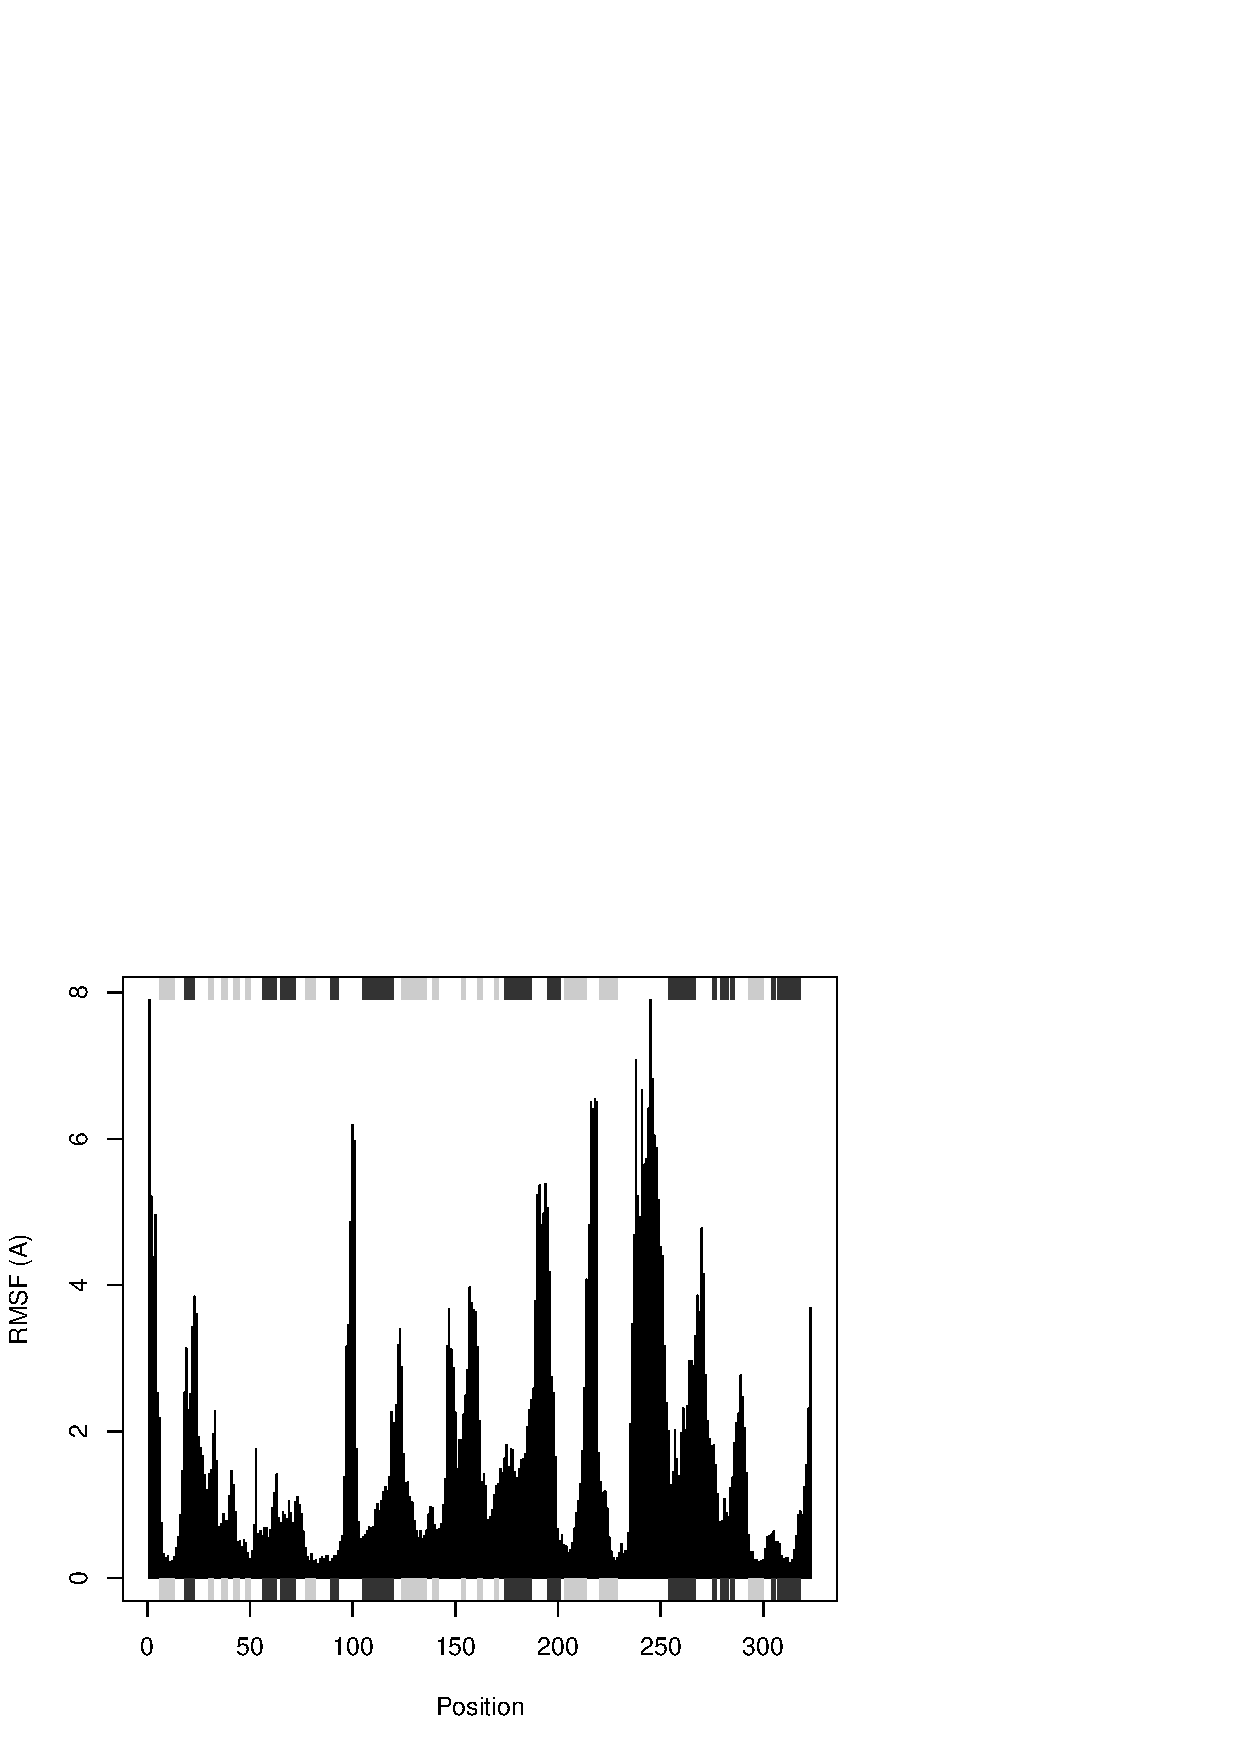
\includegraphics{figs/fig-026}
\end{center}


\paragraph{Torsion/Dihedral analysis and Difference distance matrix analysis (DDM):}
The conformation of a polypeptide or nucleotide chain can be usefully described in terms of angles of internal rotation around its constituent bonds.
\begin{Schunk}
\begin{Sinput}
> tor <- torsion.pdb(pdb)
\end{Sinput}
\end{Schunk}
\begin{center}
\begin{Schunk}
\begin{Sinput}
> plot(tor$phi, tor$psi, xlab = "phi", ylab = "psi")
\end{Sinput}
\end{Schunk}
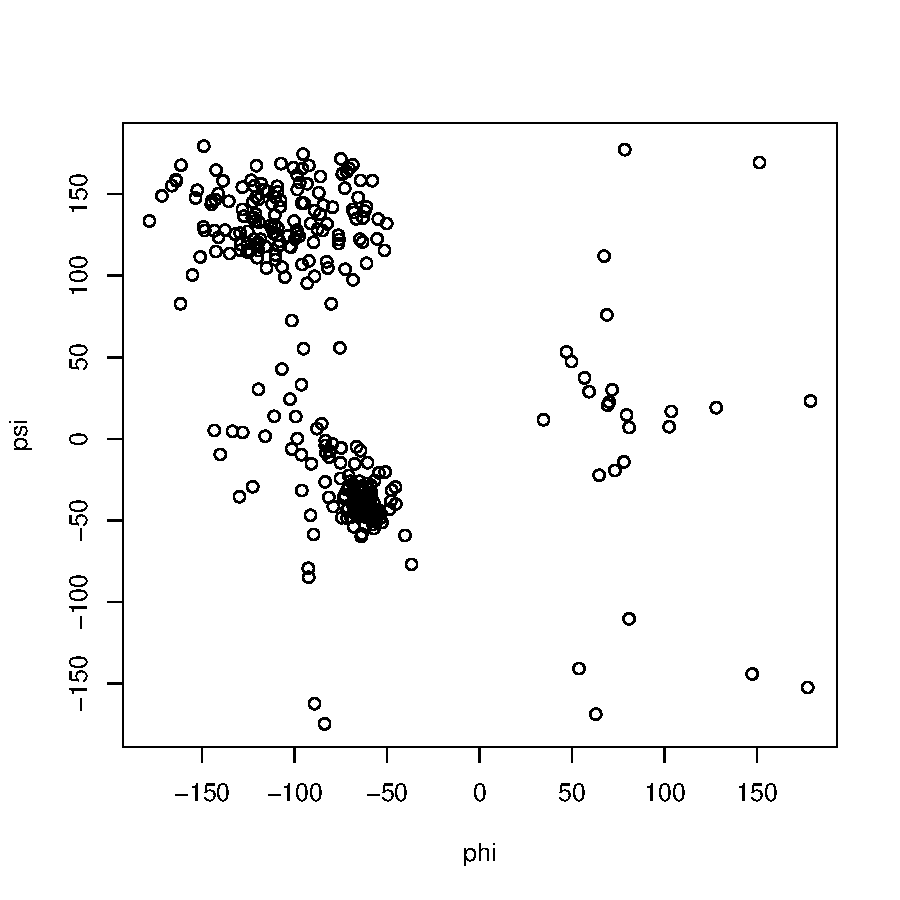
\includegraphics{figs/fig-028}
\end{center}

\begin{Schunk}
\begin{Sinput}
> a.xyz <- pdbs$xyz[(pdbs$id == "d1i5sa_"), ]
> b.xyz <- pdbs$xyz[(pdbs$id == "d1i6ia_"), ]
> gaps.xyz <- is.gap(pdbs$xyz[(pdbs$id == "d1bg2__"), ])
> gaps.res <- is.gap(pdbs$ali[(pdbs$id == "d1bg2__"), ])
> resno <- pdbs$resno[(pdbs$id == "d1bg2__"), !gaps.res]
> a <- torsion.xyz(a.xyz[!gaps.xyz], atm.inc = 1)
> b <- torsion.xyz(b.xyz[!gaps.xyz], atm.inc = 1)
> d.ab <- wrap.tor(a - b)
> a <- dm(a.xyz[!gaps.xyz])
\end{Sinput}
\begin{Soutput}
input is raw 'xyz' thus 'selection' ignored 
\end{Soutput}
\begin{Sinput}
> b <- dm(b.xyz[!gaps.xyz])
\end{Sinput}
\begin{Soutput}
input is raw 'xyz' thus 'selection' ignored 
\end{Soutput}
\begin{Sinput}
> ddm <- a - b
\end{Sinput}
\end{Schunk}

\begin{center}
\begin{Schunk}
\begin{Sinput}
> par(mfrow = c(2, 1), mar = c(4, 4, 0, 1))
> plot(resno, d.ab, typ = "h", xlab = "", ylab = "Angle")
> plot.bio3d(resno, abs(d.ab), typ = "h", sse = sse, xlab = "Residue", 
+     ylab = "Angle")
\end{Sinput}
\end{Schunk}
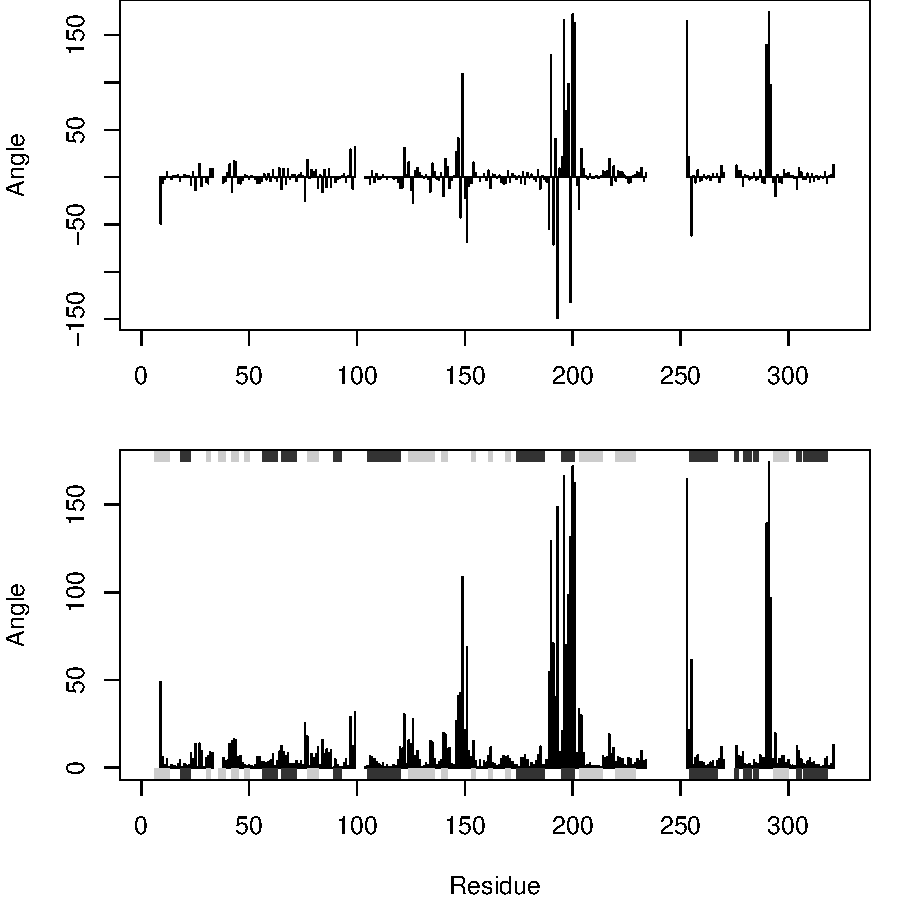
\includegraphics{figs/fig-030}

\begin{Schunk}
\begin{Sinput}
> plot(ddm, nlevels = 10, grid.col = "gray", resnum.1 = resno, 
+     resnum.2 = resno, xlab = "1i6i (positions relative to 1bg2)", 
+     ylab = "1i5s (positions relative to 1bg2)")
\end{Sinput}
\end{Schunk}
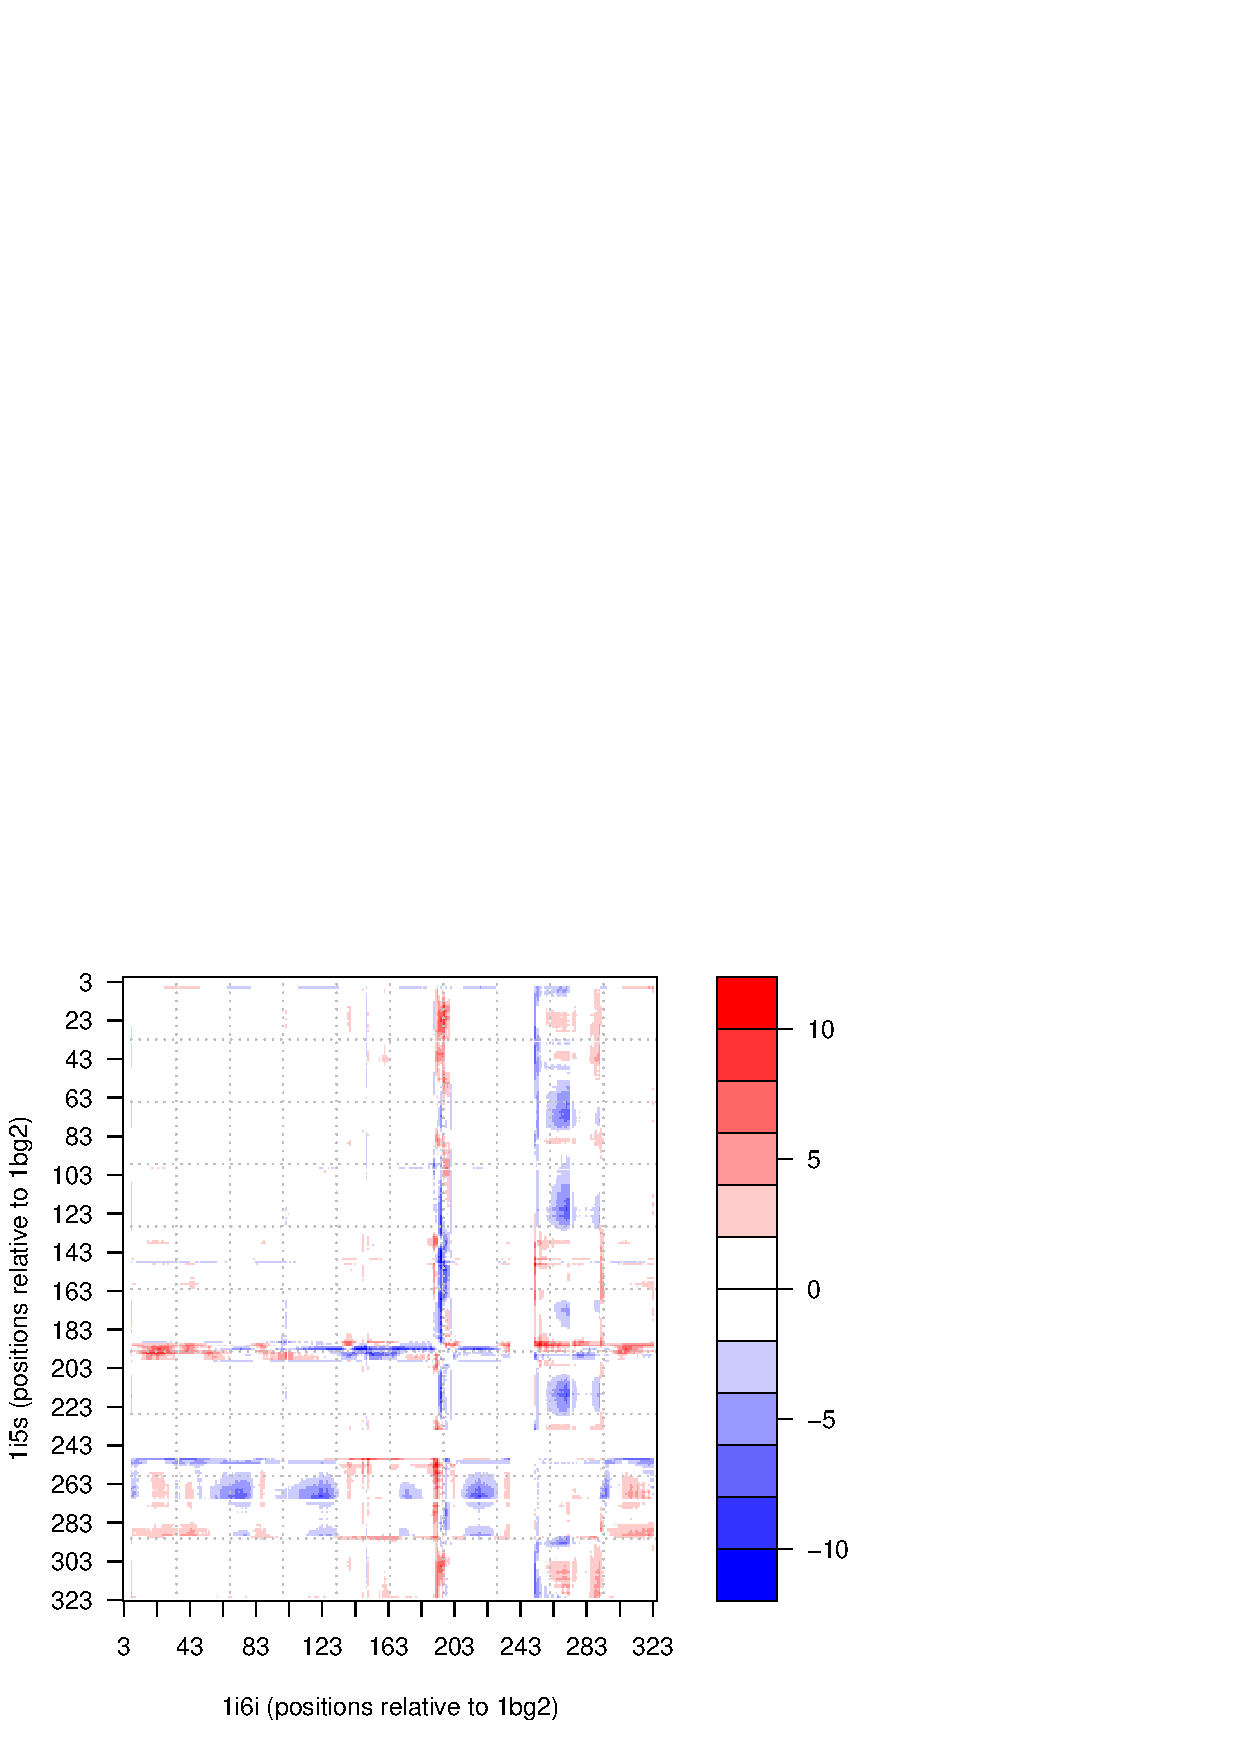
\includegraphics{figs/fig-031}
 
\end{center}















\subsection{Sequence Conservation Analysis}
The \texttt{read.fasta} and  \texttt{write.fasta} functions can be used to read and write aligned and non aligned sequences in FASTA format.  Whilst the \texttt{aln2html()} function renders a sequence alignment as coloured HTML suitable for viewing with a web browser.

\subsubsection{Sequence Alignment}
The \texttt{seqaln()} function permits the alignment of multiple sequences as obtained from the \texttt{read.fasta()}.  A simple alignment procedure for the sequences in the file \emph{unaligned.fa} would involve the commands:
\begin{Schunk}
\begin{Sinput}
> aln <- seqaln(read.fasta("unaligned.fa"))
\end{Sinput}
\end{Schunk}

\subsubsection{Residue Conservation Analysis}
To assess the level of sequence conservation at each position in
an alignment, the \emph{similarity}, \emph{identity}, and \emph{entropy} per position can be calculated with the \texttt{conserv()} function.

The \emph{similarity} is defined as the average of the similarity
scores of all pairwise residue comparisons for that position in
the alignment, where the similarity score between any two residues
is the score value between those residues in the chosen
substitution matrix.

The \emph{identity} i.e. the preference for a specific amino acid to be
found at a certain position, is assessed by averaging the identity
scores resulting from all possible pairwise comparisons at that
position in the alignment, where all identical residue comparisons
are given a score of 1 and all other comparisons are given a value
of 0.

\emph{Entropy} is based on Shannon's information entropy. See the
\texttt{entropy} function for further details.

\begin{Schunk}
\begin{Sinput}
> aln <- read.fasta(system.file("examples/kinesin_xray.fa", package = "bio3d"))
> sim <- conserv(x = aln$ali, method = "similarity", sub.matrix = "bio3d")
\end{Sinput}
\end{Schunk}

\begin{center}
\begin{Schunk}
\begin{Sinput}
> sse <- dssp(pdb, resno = FALSE)
> plot.bio3d(sim[!is.gap(aln$ali[1, ])], sse = sse, xlab = "Residue", 
+     ylab = "Similarity")
\end{Sinput}
\end{Schunk}
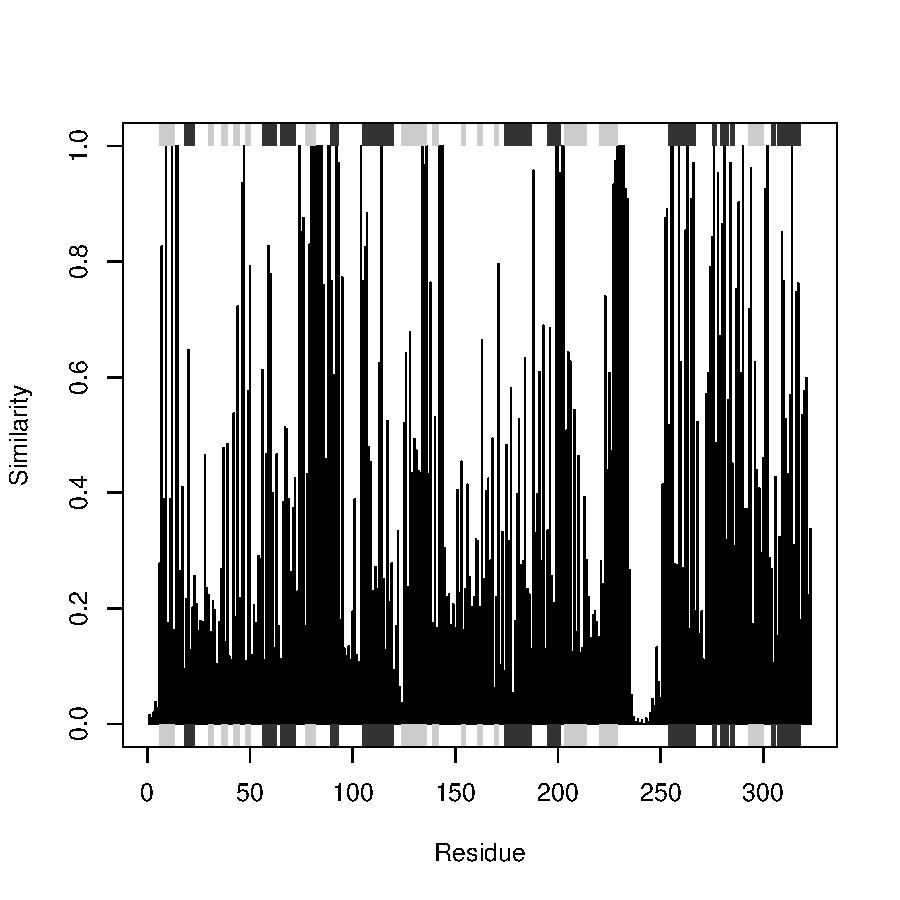
\includegraphics{figs/fig-034}
\end{center}



\begin{Schunk}
\begin{Sinput}
> aln <- read.fasta(system.file("examples/kinesin_xray.fa", package = "bio3d"))
> write.fasta(seqs = aln$ali[, 379:385], file = "eg.fa")
> aln2html(aln, append = FALSE, file = "eg.html")
> aln2html(aln, colorscheme = "ent", file = "eg.html")
\end{Sinput}
\end{Schunk}


\subsubsection*{Identity, Clustering, Consensus, etc.}

Pairwise identity analysis
dm plot, histogram, ide.filter


Determine the consensus sequence for a given alignment at a given identity cutoff value.

\begin{Schunk}
\begin{Sinput}
> con <- consensus(aln$ali, cutoff = 0.6)
\end{Sinput}
\end{Schunk}
Quantifies residue conservation in a given protein sequence
alignment by calculating the degree of amino acid variability in
each column of the alignment.

\begin{Schunk}
\begin{Sinput}
> con.sim <- conserv(x = aln$ali, method = "similarity", sub.matrix = "bio3d")
\end{Sinput}
\end{Schunk}
plot conservation 





\subsection{Basic Trajectory Analysis}
Read a CHARMM/X-PLOR/NAMD trajectory file
\begin{Schunk}
\begin{Sinput}
> trtfile <- system.file("examples/hivp.dcd", package = "bio3d")
> trj <- read.dcd(trtfile)
\end{Sinput}
\begin{Soutput}
Created by DCD plugin
REMARKS Created 23 May, 2006 at 11:39
 NATOM = 198 
 NFRAME= 351 
 ISTART= 0 
 last  = 351 
 nstep = 351 
 nfile = 351 
 NSAVE = 1 
 NDEGF = 0 
 version 24 
Reading (x100)...done
\end{Soutput}
\end{Schunk}

Read the starting PDB file to determine atom correspondence
\begin{Schunk}
\begin{Sinput}
> pdbfile <- system.file("examples/hivp.pdb", package = "bio3d")
> pdb <- read.pdb(pdbfile)
\end{Sinput}
\end{Schunk}

\subsubsection*{Superposition, RMSD, RMSF, PCA, etc.}
Fit trj on PDB based on residues 23 to 31 and 84 to 87 in both chains
\begin{Schunk}
\begin{Sinput}
> inds <- atom.select(pdb, "///23:31,84:87///CA/")
\end{Sinput}
\begin{Soutput}
      segid chain resno         resid eleno elety
Stest ""    ""    "23:31,84:87" ""    ""    "CA" 
Natom "198" "198" "26"          "198" "198" "198"
 *  Selected a total of: 26 intersecting atoms  *
\end{Soutput}
\begin{Sinput}
> fit.xyz <- fit.xyz(pdb$xyz, trj, fixed.inds = inds$xyz, mobile.inds = inds$xyz)
\end{Sinput}
\end{Schunk}
RMSD of trj frames from PDB
\begin{Schunk}
\begin{Sinput}
> r <- rmsd(a = pdb, b = fit.xyz)
\end{Sinput}
\end{Schunk}


PCA of trj
\begin{Schunk}
\begin{Sinput}
> pc.trj <- pca.xyz(fit.xyz)
\end{Sinput}
\end{Schunk}
Overview of PCA results with \texttt{plot.pca}:

Cluster along pc1-2 planes
\begin{Schunk}
\begin{Sinput}
> hc <- hclust(dist(pc.trj$z[, 1:2]))
> grps <- cutree(hc, k = 2)
\end{Sinput}
\end{Schunk}

\begin{center}
\begin{Schunk}
\begin{Sinput}
> plot(pc.trj, col = c("red", "blue")[grps])
\end{Sinput}
\end{Schunk}
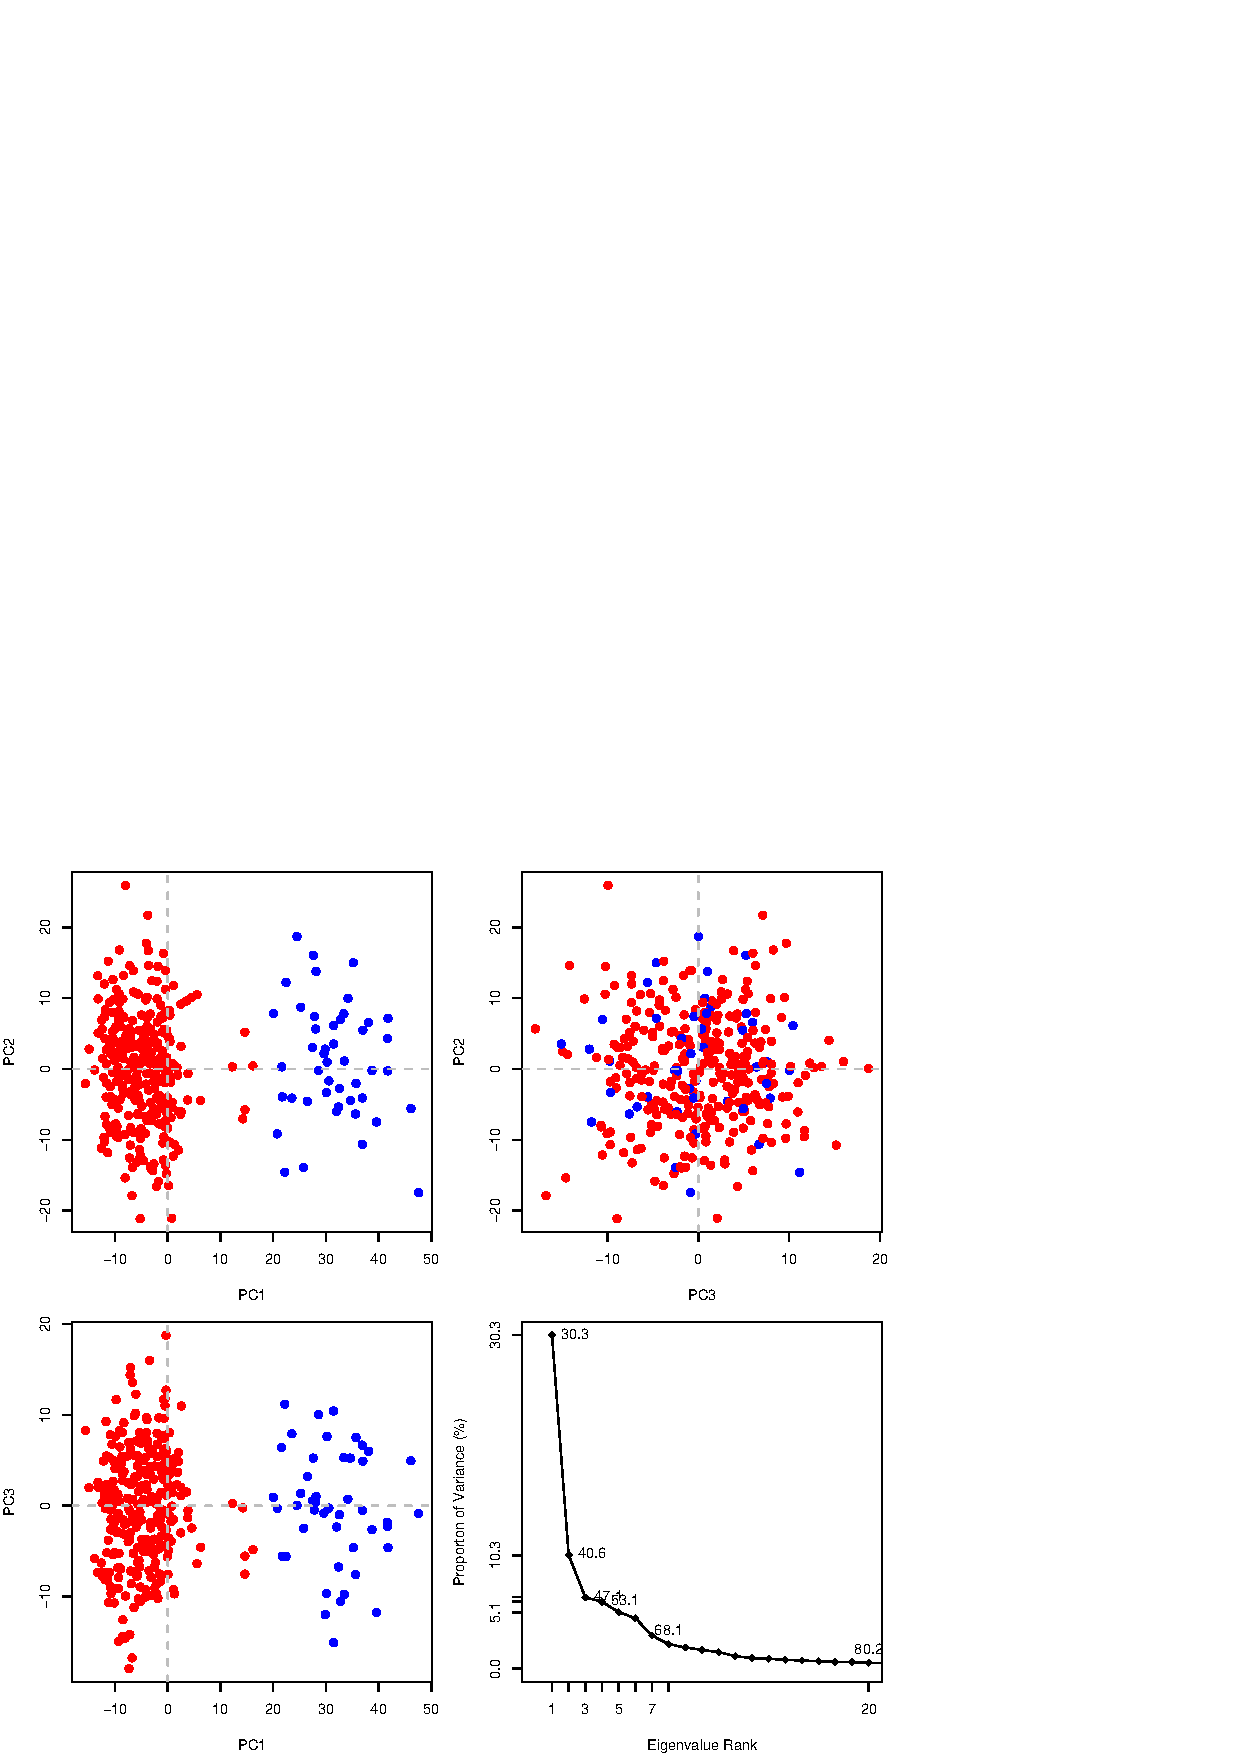
\includegraphics{figs/fig-044}
\end{center}


Residue contributions to the first principal component

\begin{center}
\begin{Schunk}
\begin{Sinput}
> plot.bio3d(pc.trj$au[, 1], xlab = "Residue", ylab = "PC1 (A)")
\end{Sinput}
\end{Schunk}
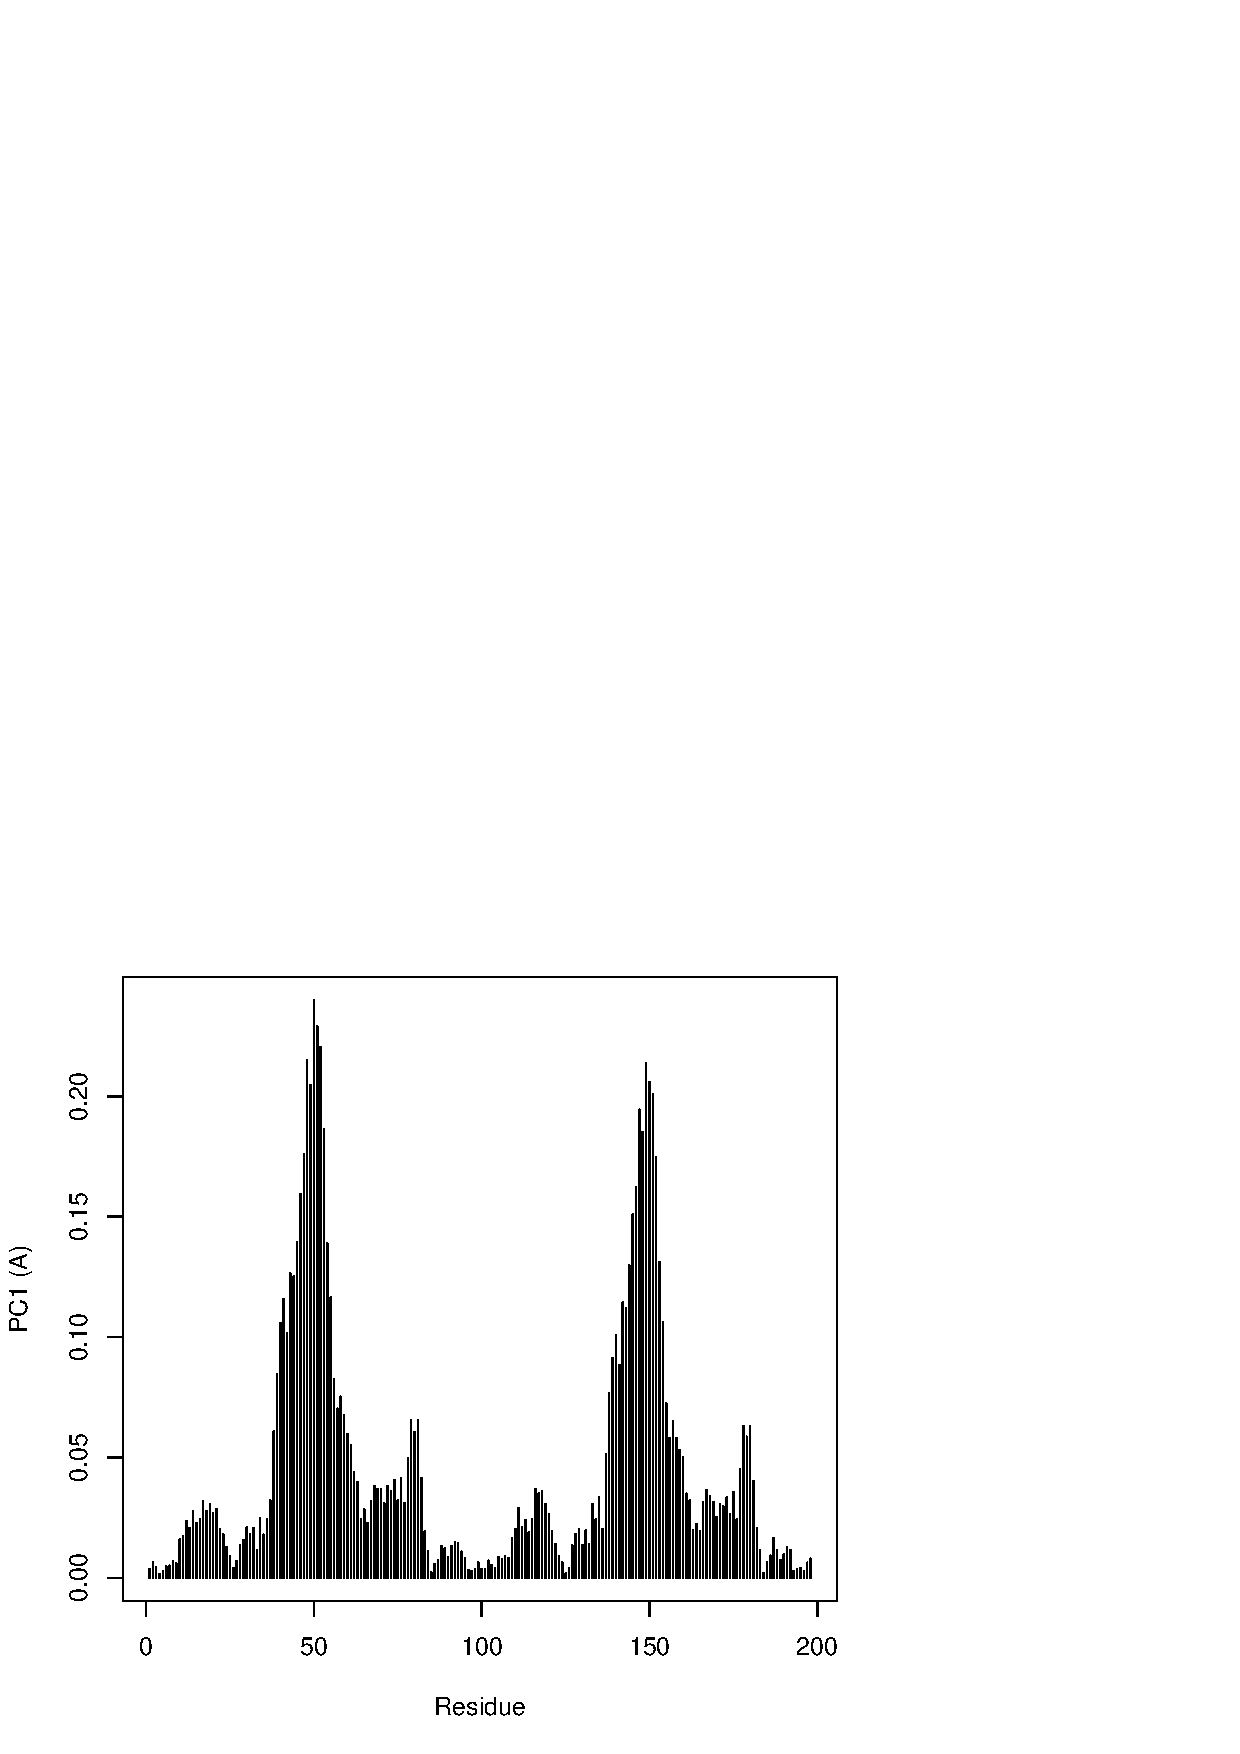
\includegraphics{figs/fig-045}
\end{center}

Write PC trajectory
\begin{Schunk}
\begin{Sinput}
> a <- mktrj.pca(pc.trj, pc = 1, file = "pc1_trj.pdb")
\end{Sinput}
\end{Schunk}


Cross-Correlation Analysis
To be finished.

A more detailed discussion will be the subject of a future vignette.


\subsection*{Session Info}
\begin{Schunk}
\begin{Sinput}
> toLatex(sessionInfo())
\end{Sinput}
\begin{Soutput}
\begin{itemize}
  \item R version 2.7.2 (2008-08-25), \verb|x86_64-unknown-linux-gnu|
  \item Locale: \verb|LC_CTYPE=en_US.UTF-8;LC_NUMERIC=C;LC_TIME=en_US.UTF-8;LC_COLLATE=en_US.UTF-8;LC_MONETARY=C;LC_MESSAGES=en_US.UTF-8;LC_PAPER=en_US.UTF-8;LC_NAME=C;LC_ADDRESS=C;LC_TELEPHONE=C;LC_MEASUREMENT=en_US.UTF-8;LC_IDENTIFICATION=C|
  \item Base packages: base, datasets, graphics, grDevices, methods,
    stats, utils
  \item Other packages: bio3d~1.0-6
  \item Loaded via a namespace (and not attached): tools~2.7.2
\end{itemize}
\end{Soutput}
\end{Schunk}

\begin{thebibliography}{9}


\bibitem[Grant \emph{et al.}, 2006]{grant06}
Grant, B.J. and Rodrigues, A.P.D.C and Elsawy, K.M. and Mccammon, A.J. and Caves, L.S.D. (2006)
\textbf{Bio3d: an R package for the comparative analysis of protein structures.}
\emph{Bioinformatics},
\textbf{22}, 2695--2696.


\bibitem[Grant \emph{et al.}, 2007]{grant07}
Grant, B.J. and Mccammon, A.J. and Caves, L.S.D. and Cross, R.A. (2007)
\textbf{Multivariate Analysis of Conserved Sequence-Structure Relationships in Kinesins: Coupling of the Active Site and a Tubulin-binding Sub-domain.}
\emph{J. Mol. Biol.},
\textbf{5}, 1231--1248


\bibitem[Fischer and Karplus, 1992]{cpr}
Fischer, S. and Karplus, M. (1992) 
\textbf{Conjugate peak refinement: an algorithm for finding reaction paths and accurate transition states in systems with many degrees of freedom.}
\emph{Chem. Phys. Lett}, \textbf{194}, 252--261


\bibitem[Hayward and Berendsen, 1989]{dyndom}
Hayward, S. and Berendsen, H. (1998) 
\textbf{Systematic analysis of domain motions in proteins from conformational change: new results on citrate synthase and T4 lysozyme.}
\emph{Proteins}, \textbf{30}, 144--154


\bibitem[Humphrey \emph{et al.}, 1996]{vmd}
Humphrey, W., et al. (1996) 
\textbf{VMD: visual molecular dynamics.}
\emph{J. Mol. Graph}, \textbf{14}, 33--38



\end{thebibliography}




\end{document}

